% manuscript produces a one-column, double-spaced document:
%\documentclass[12pt,preprint]{aastex}
\documentclass[manuscript]{aastex6}
%\documentclass[iop]{emulateapj}

% preprint2 produces a double-column, single-spaced document:
%\documentclass[preprint2]{aastex}

%Packages
%\usepackage[colorlinks=true,linkcolor=blue,citecolor=blue]{hyperref}

\usepackage{natbib}
\usepackage[caption=false]{subfig}
\usepackage{amsmath,amssymb}
\newcommand{\vdag}{(v)^\dagger}
\newcommand{\degree}{$^\circ$}
\newcommand{\vtan}{$V_{tan}$}
\newcommand{\kms}{km~s$^{-1}$}
\newcommand{\msun}{M$_{\sun}$}
\newcommand{\rjup}{R$_{Jup}$}
\newcommand{\ldl}{$\lambda/{\Delta}{\lambda}$}
\newcommand{\lsun}{L$_{\sun}$}
\newcommand{\lbol}{$\log_{10}{L_{bol}/L_{\sun}}$}
\newcommand{\teff}{T$_{eff}$}
\newcommand{\logg}{$\log{g}$}
\newcommand{\fsed}{$f_{sed}$}
\newcommand{\kzz}{$K_{zz}$}
\newcommand{\meth}{CH$_4$}
\newcommand{\wat}{H$_2$O}
\newcommand{\sha}{2MASS~J0835$-$0819}
\newcommand{\shb}{2MASS~J1821+1414}

\slugcomment{To be submitted to ApJ/AJ}


\shorttitle{Spectral Variability of L Dwarfs}
\shortauthors{Schlawin et al.}


\begin{document}


\title{Supplement to Spectral Variability of Two Rapidly Rotating Brown Dwarfs: \\2MASS~J08354256$-$0819237 and 2MASS~J18212815+1414010}

%% Use \author, \affil, and the \and command to format
%% author and affiliation information.
%% Note that \email has replaced the old \authoremail command
%% from AASTeX v4.0. You can use \email to mark an email address
%% anywhere in the paper, not just in the front matter.
%% As in the title, use \\ to force line breaks.

\author{E. Schlawin\altaffilmark{1,2}, Adam J.\ Burgasser\altaffilmark{2,3}, J. Gizis\altaffilmark{4}, T. Karalidi\altaffilmark{1}, \and J. Teske\altaffilmark{5}}

\altaffiltext{1}{Steward Observatory, Tucson AZ 85721 \email{eas342@email.arizona.edu}}
\altaffiltext{2}{Visiting Astronomer at the Infrared Telescope Facility, which is operated by the University of Hawaii under contract NNH14CK55B with the National Aeronautics and Space Administration}
\altaffiltext{3}{Center for Astrophysics and Space Science, University of California San Diego, La Jolla, CA 92093, USA}
\altaffiltext{4}{Department of Physics and Astronomy, University of Delaware, Newark, DE 19716, USA}
\altaffiltext{5}{Carnegie Observatories, 813 Santa Barbara Street, Pasadena, CA 91101, USA}

\begin{abstract}
Supplementary Information
\end{abstract}


\keywords{techniques: spectroscopic -- stars: atmospheres -- stars: brown dwarfs -- stars: individual (\objectname{2MASS J08354256-0819237}, \objectname{2MASS J18212815+1414010}) -- stars: late-type -- stars: variables: general}


\section{Color-Magnitude Diagram}

Figure \ref{fig:CMD} shows the color magnitude diagram from the sample of brown dwarfs in \citet{dupuy2012ltparallax}, which includes 2MASS J0835 but not 2MASS J1821.
We highlight these two brown dwarfs to be contrasted with the rest of the population.

\begin{figure}
\begin{centering}
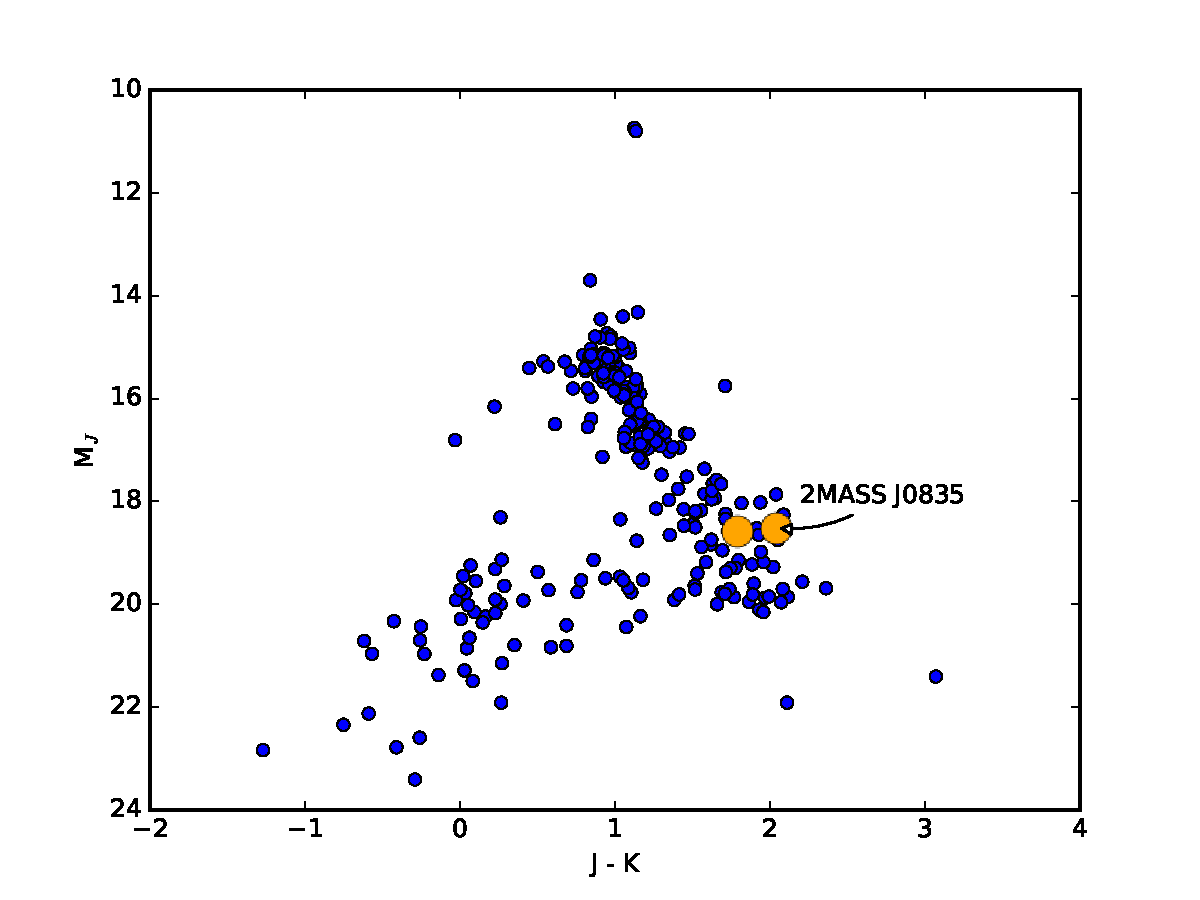
\includegraphics[width=0.5\textwidth]{color_mag.pdf}
\caption{Color-Magnitude diagram from \citet{dupuy2012ltparallax}. We added 2MASS J1821 using Simbad magnitudes and parallaxes.}\label{fig:CMD}
\end{centering}
\end{figure}

\pagebreak
\section{Example Posterior Distributions}
[DO WE NEED MORE TEXT IN THIS SECTION EXPLAINING EACH FIGURE?]
\subsection{Time Series}
In Figure \ref{fig:postCosfit}, we show the posterior distributions of a sinusoidal model (Equation \ref{eq:cosfit}) fit to the data using \texttt{emcee} \citep{foreman-mackey2013emcee} for an example wavelength bin of 1.08~$\mu$m.
This wavelength bin is one of the high amplitude fits that is relatively unaffected by telluric contamination.
In this example, we input photon noise only.
We impose priors on the amplitude $A_1 > 0$, $|t_t| < 6 hr$ (to avoid multiple periodic solutions) and that the period $0 < \tau < 6 hr$ so that the periodicity is shorter than the observation window length.
The model parameters are close to Gaussian and the only visible correlation is between the time offset, $t_1$, and the rotation period $\tau$.
The maximum likelihood solution is shown in Figure \ref{fig:model2Cosfit} and has a chi-squared per degree of freedom ($\bar{\chi^2}$) of 12.1

\begin{figure}
\begin{centering}
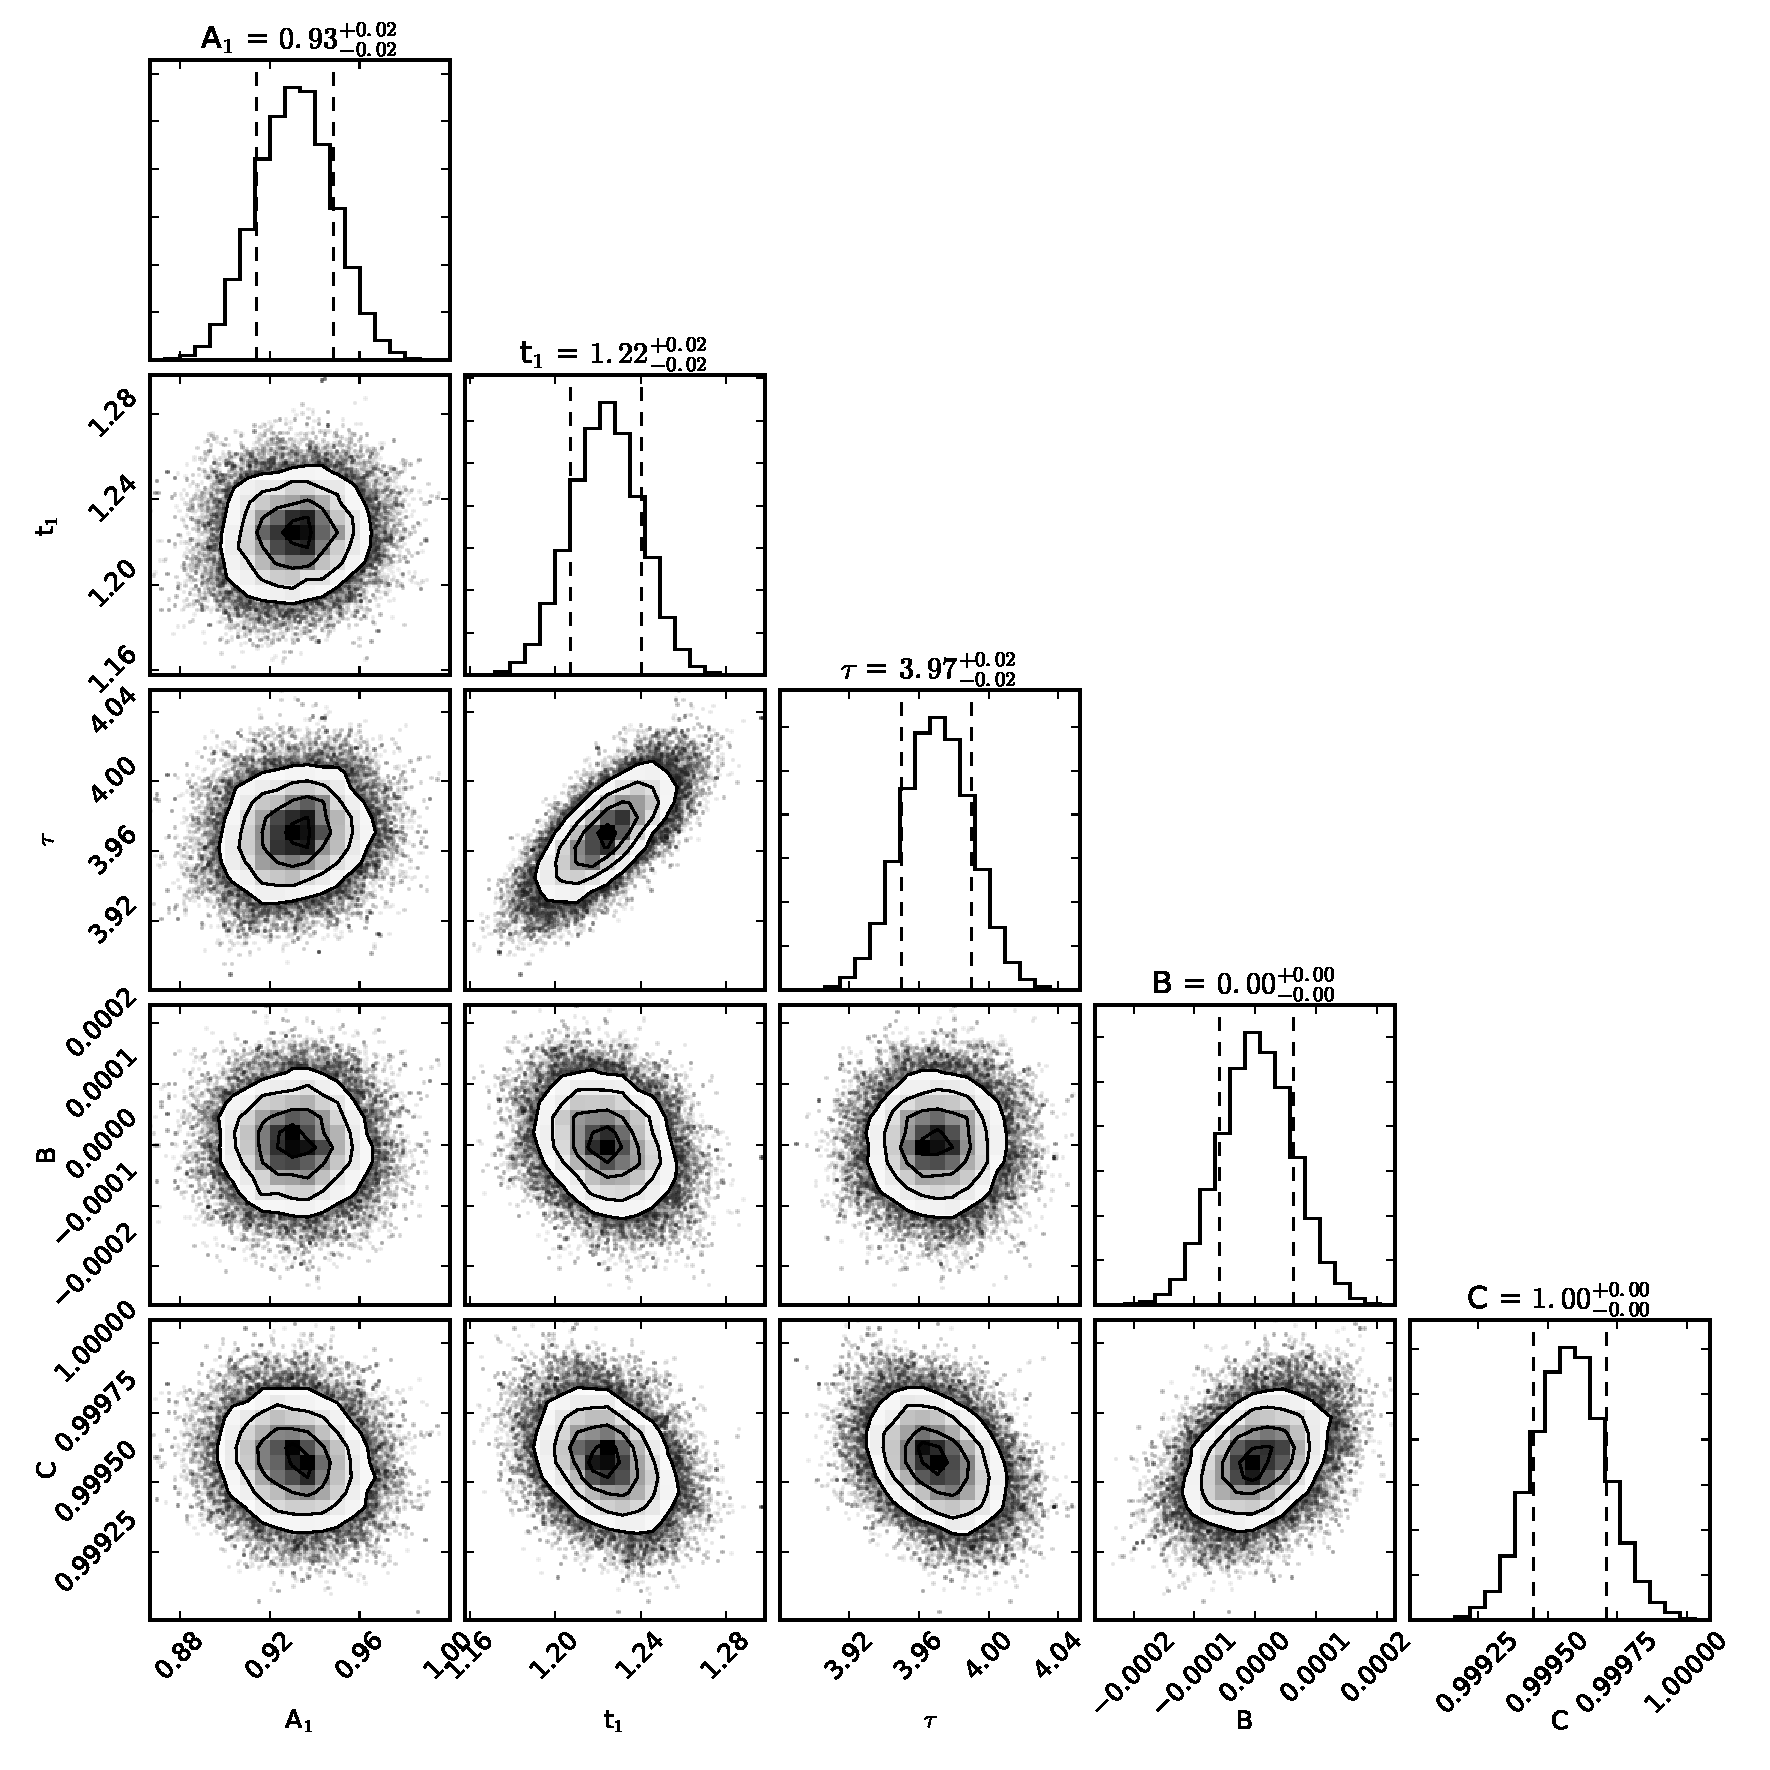
\includegraphics[width=0.5\textwidth]{corner_example.pdf}
\caption{Example posterior distributions for an MCMC fit to the time series using Equation \ref{eq:cosfit} for the wavelength bin 1.08~$\mu$m.
Amplitude, $A_1$ is in percent, the time offset $t_1$ is in hours, the period of oscillation, $\tau$, is in units of hours, B is in units of fraction of flux per hour and C is the offset constant in fraction (not percent).
We only input photon counting and read noise statistics for the errors.
This is likely and underestimate for the uncertainty in the time series.
}\label{fig:postCosfit}
\end{centering}
\end{figure}

Since Equation \ref{eq:cosfit} is a poor fit to the data, as visible in Figure \ref{fig:model2Cosfit}, we also explore models with additional sinusoidal frequencies.
In the multiple term model, we add cosine functions at $n$ times the frequency:
\begin{equation}\label{eq:cosfitMultiTerm}
F(t) = B t + C + A_1 \cos(2 \pi (t - t_1)/\tau) + A_2 \cos(4 \pi (t - t_2)/\tau) + A_n \cos(2 n \pi (t - t_n)/\tau) +  ...
\end{equation}
Now there are $n$ amplitude parameters $A_n$ and $n$ time offset parameters $t_n$.
Figure \ref{fig:model2Cosfit} shows the best fit compared to the data for 2 term and 3 term sinusoidal fits.
We assume the same priors as the 1 term sinusoidal fit with  $A_n > 0$.
For the time offsets, we restrict the range to be $\pm$ 4 hr / $n$.
The multiple term model appear visually to fit the data well.
However, the $\bar{\chi^2}$ are still 7.9 and 7.4, so it is not the expected 1.0.
However, the error bars are underestimated when only including photon and read noise components.
With exoplanet light curves, the standard deviation of the out-of-transit baseline flux can be used as an estimate for errors. With the brown dwarf rotation light curves, there is no flat baseline over which to measure error levels.

\begin{figure}
\begin{centering}
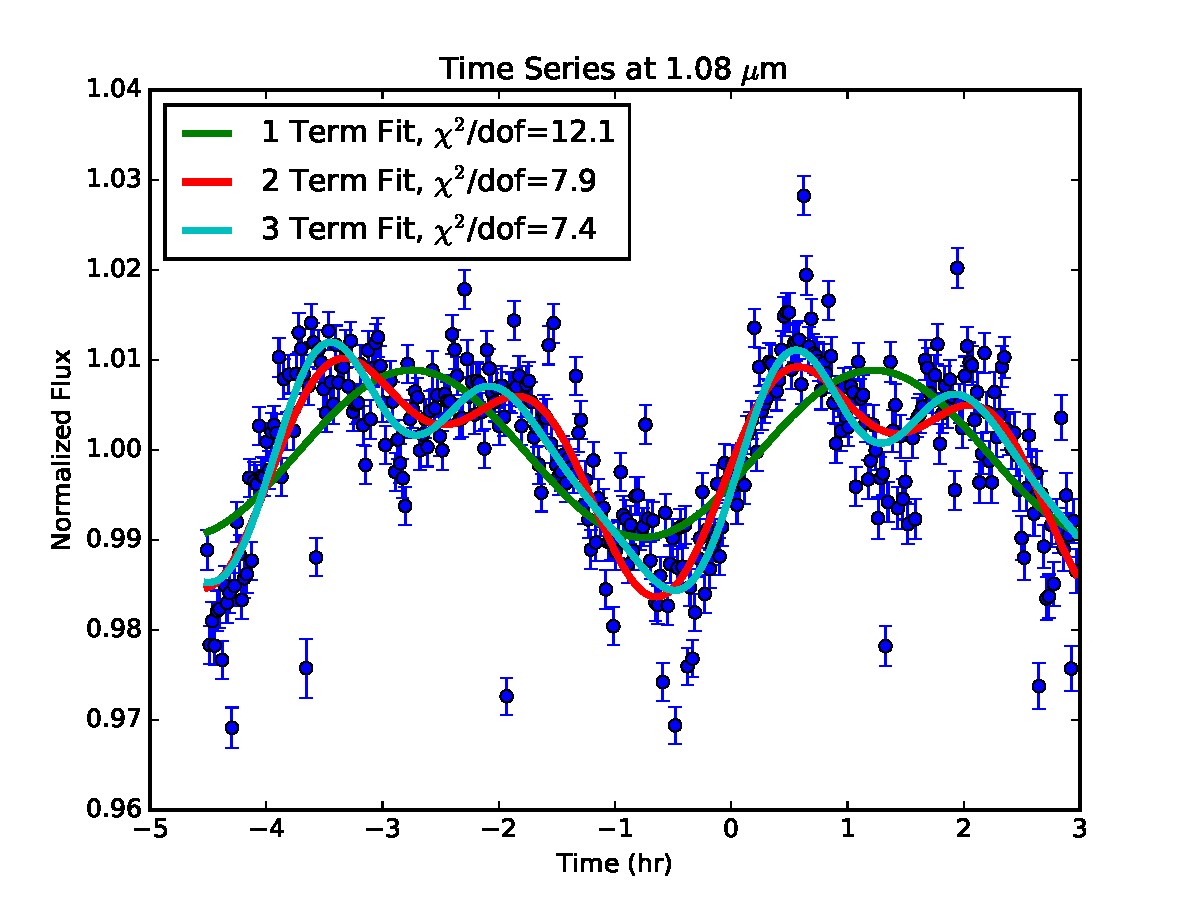
\includegraphics[width=0.5\textwidth]{best_fit_multi_terms.pdf}
\caption{A zoom-in on on the time series of 2MASS J1821 for the wavelength bin 1.08~$\mu$m. Error bars are shown for photon and read noise. We plot a best-fit models using a single cosine term (green, $\bar{\chi^2}$ = 12.1). Additional terms improve the fits to the data and the $\bar{\chi^2}$.}\label{fig:model2Cosfit}
\end{centering}
\end{figure}


\begin{figure}
\begin{centering}
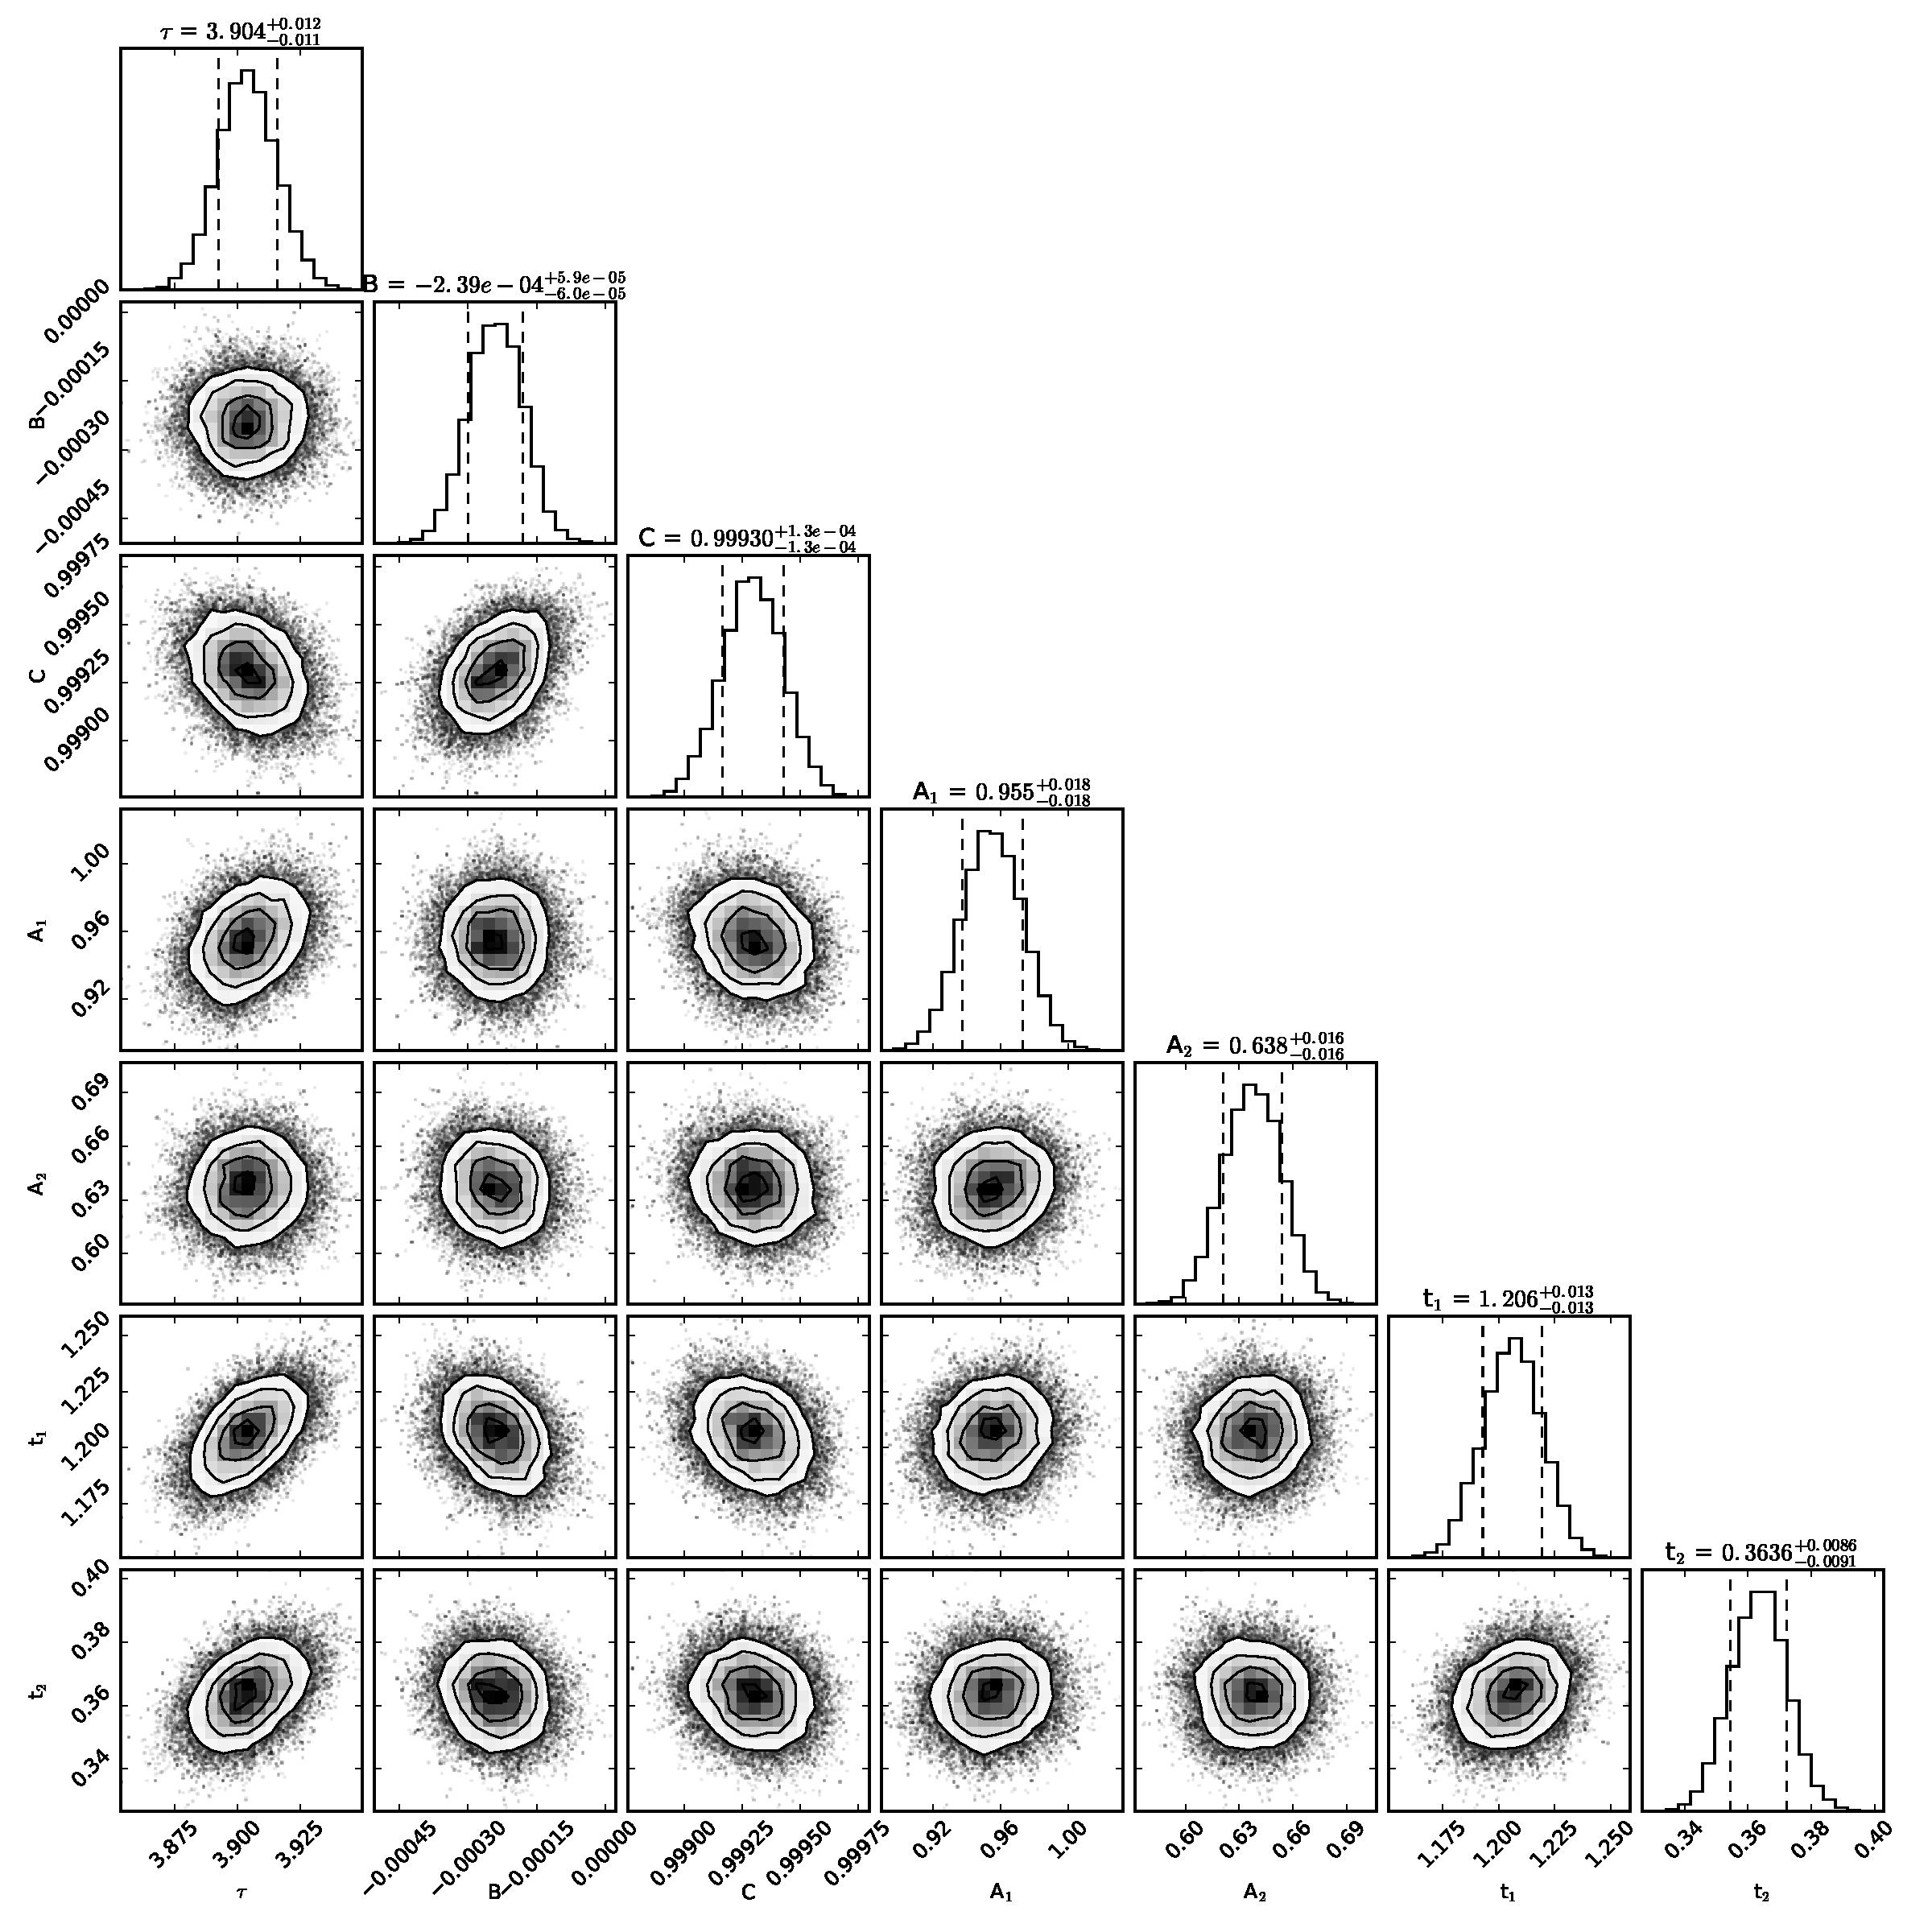
\includegraphics[width=0.7\textwidth]{corner_fit_2term.pdf}
\caption{Example posterior distributions for an MCMC fit to the time series using Equation \ref{eq:cosfitMultiTerm} for 2 terms.
Again, there is little correlation between the posteriors for the different parameters. {\it Right} Same figure, but with 3 cosine terms.}\label{fig:post2Cosfit}
\end{centering}
\end{figure}


\begin{figure}
\begin{centering}
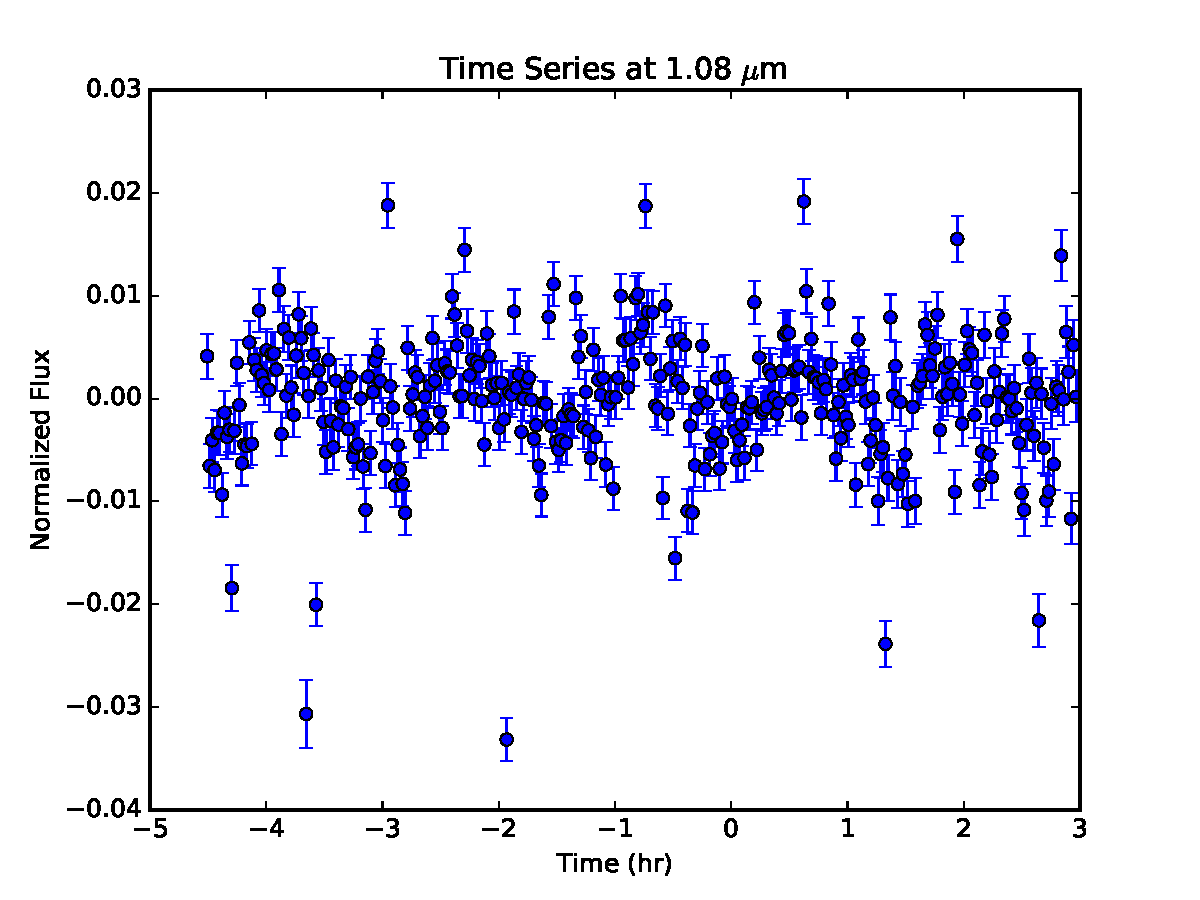
\includegraphics[width=0.48\textwidth]{residual_2term_1080nm.pdf}
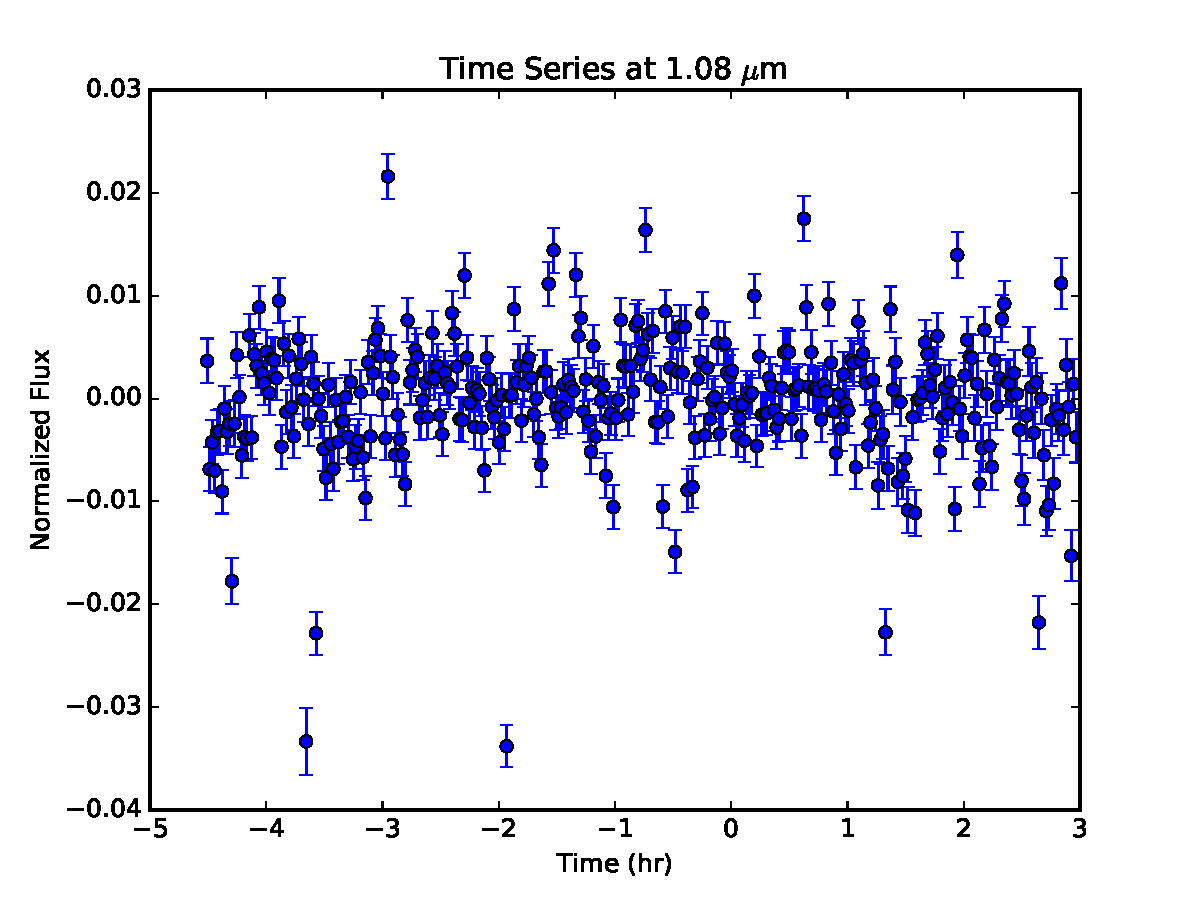
\includegraphics[width=0.48\textwidth]{residual_3term_1080nm.pdf}
\caption{Residuals after subtracting the maximum likelihood two-term model from Equation \ref{eq:cosfitMultiTerm} from the data.  We show the residuals when using a 2 term model (left) and a 3 term model (right). The standard deviation of the residuals is 0.6\% whereas the error from photon counting statistics is 0.2\%.}\label{fig:resid2Cosfit}
\end{centering}
\end{figure}

\begin{figure}
\begin{centering}
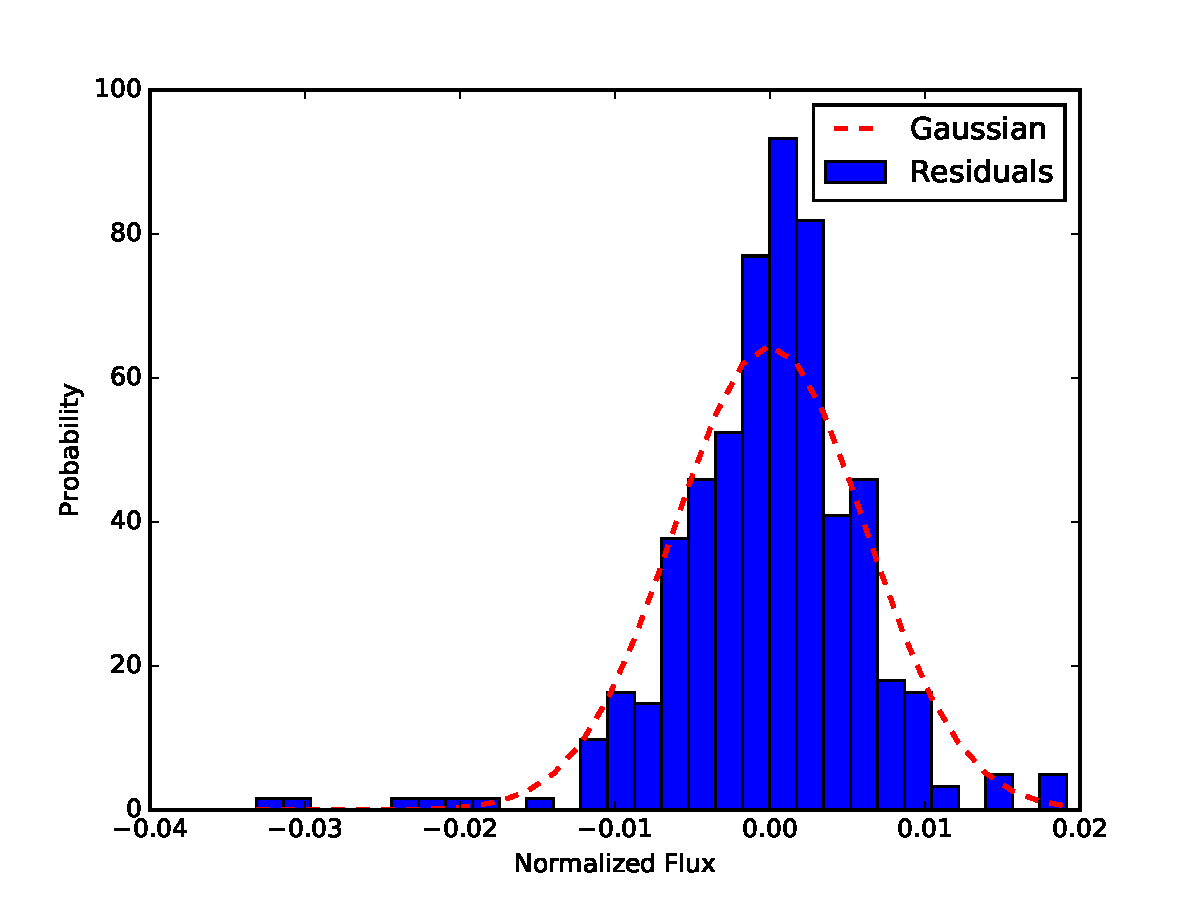
\includegraphics[width=0.5\textwidth]{histo_resids.pdf}
\caption{Histogram of residuals after subtracting the maximum likelihood model from Equation \ref{eq:cosfitMultiTerm} from the data with 2 terms.}\label{fig:histoResid2Cosfit}
\end{centering}
\end{figure}


\clearpage
\pagebreak
\subsection{Amplitude Spectrum}

We also use \texttt{emcee} to fit the amplitude spectrum of 2MASS J1821 using the two temperature surface model in Section \label{sec:spotModel} with Equation \ref{eq:twoTempAmp}.

\begin{figure}
\begin{centering}
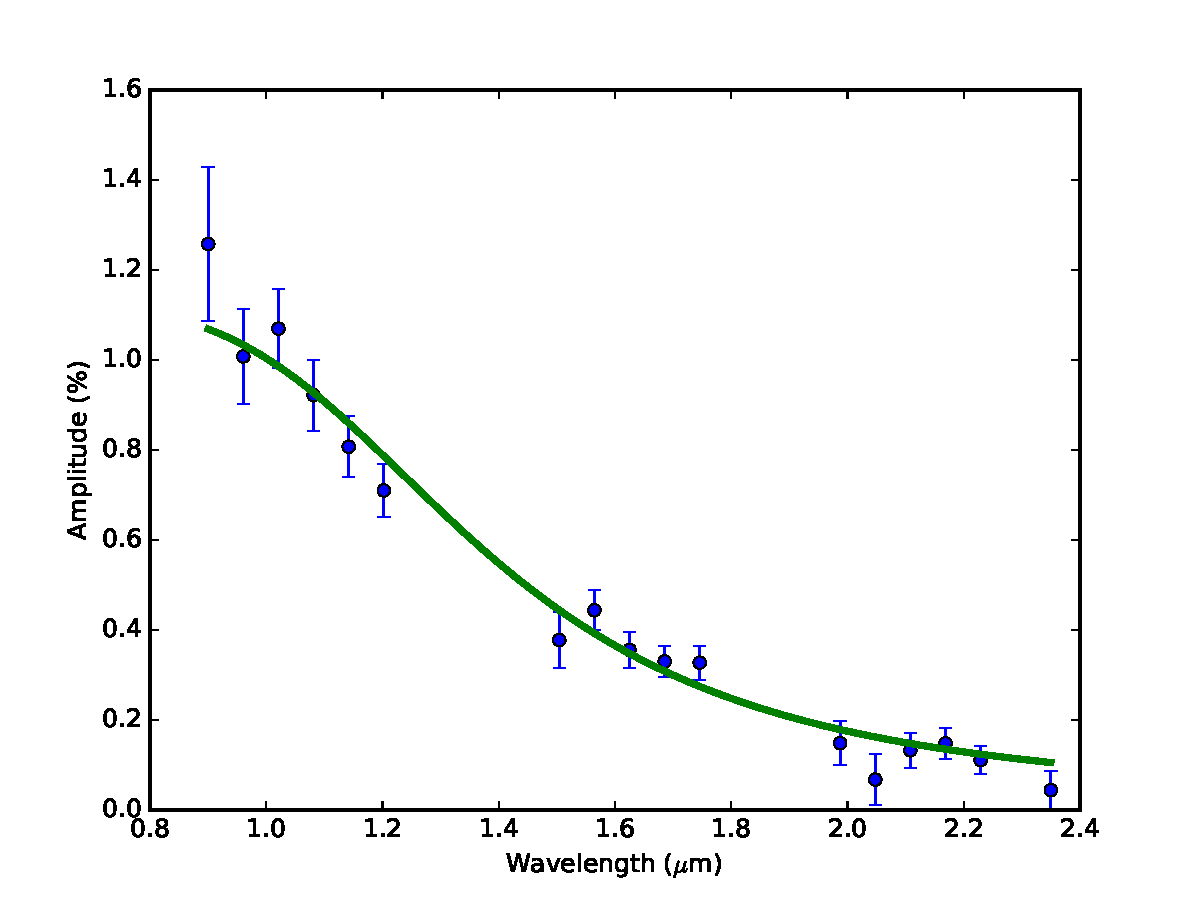
\includegraphics[width=0.5\textwidth]{best_fit_spec_2temp.pdf}
\caption{We repeat the amplitude spectrum of 2MASS J1821 from Figure \ref{fig:ampspec1821tdiff}, which excludes the wavelengths contaminated by telluric absorption.
We show a maximum likelihood model spectrum, which has a $\chi^2$ per degree of freedom of 1.16.}\label{fig:ML2Tempfit}
\end{centering}
\end{figure}

\begin{figure}
\begin{centering}
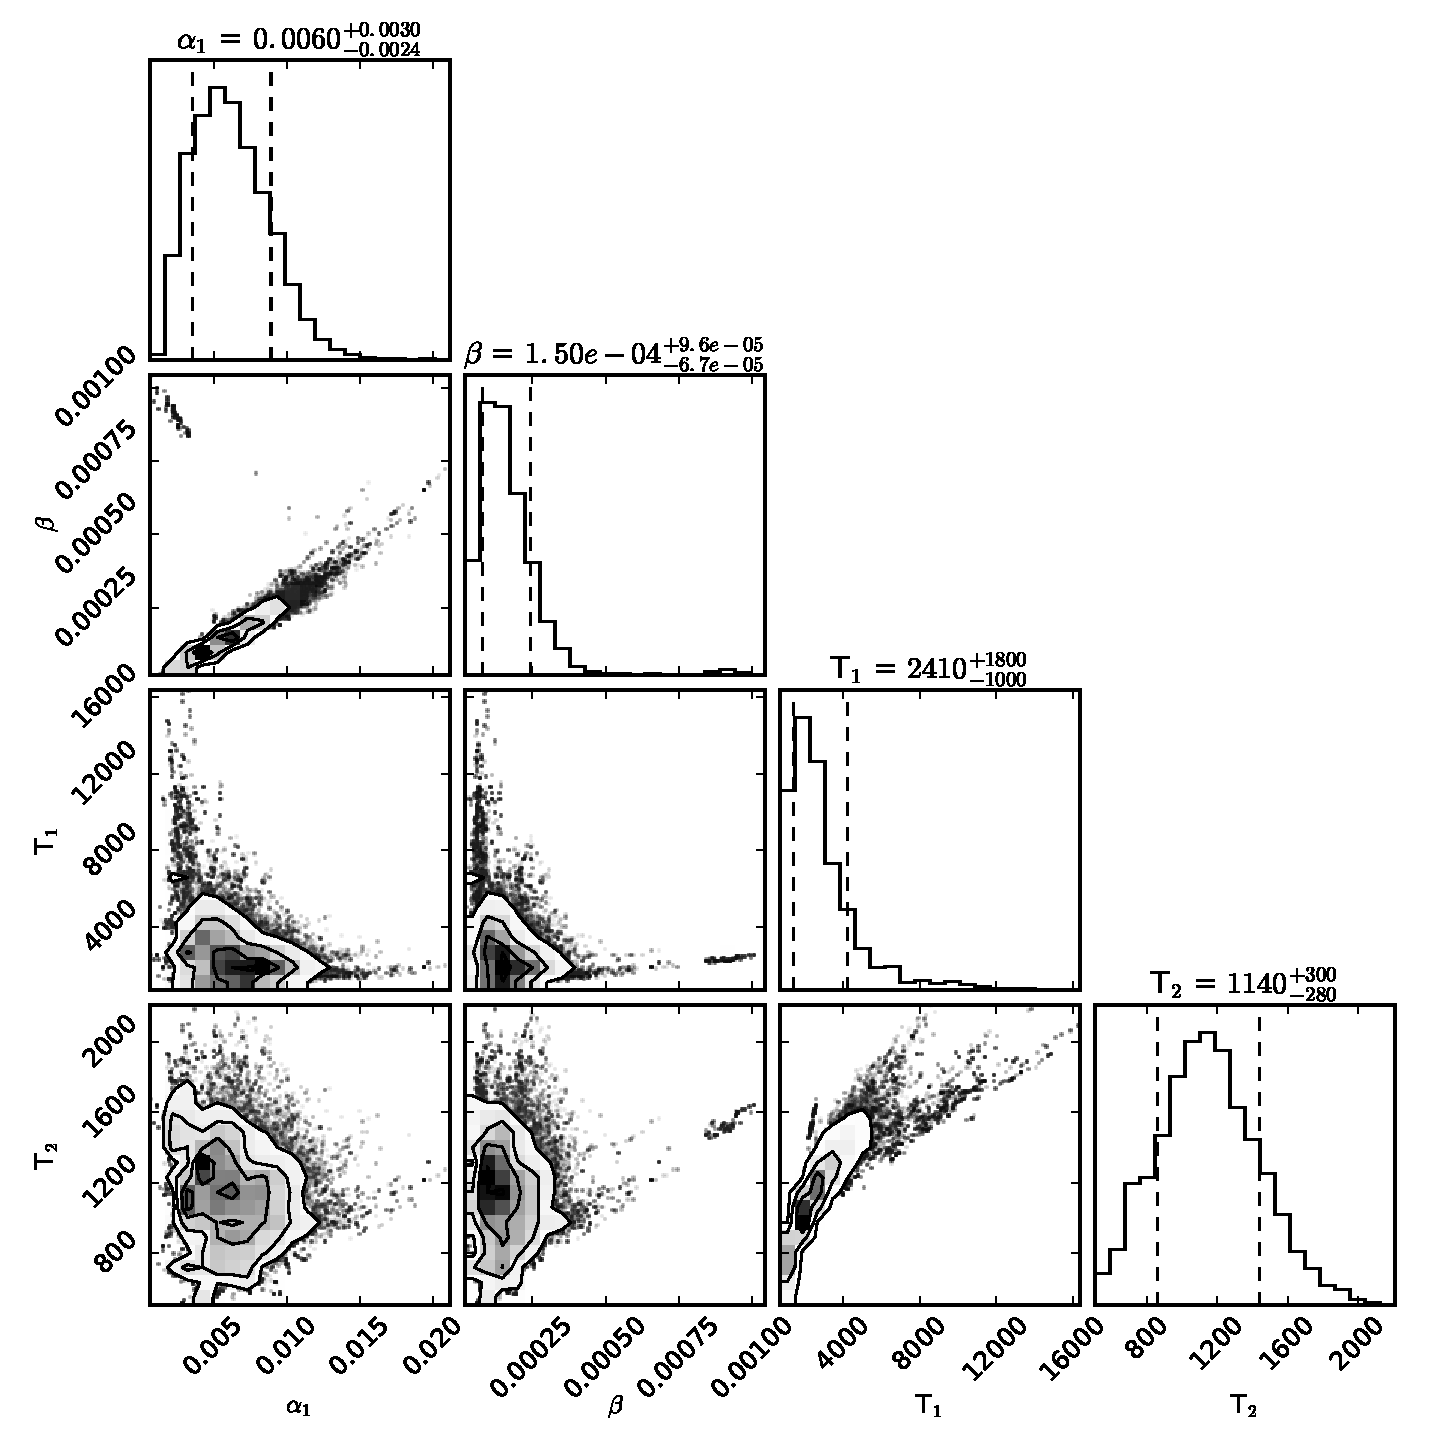
\includegraphics[width=0.5\textwidth]{corner_fit_2temp.pdf}
\caption{Example posterior distributions for an MCMC fit to the spectra using Equation \ref{eq:twoTempAmp}.}\label{fig:post2Tempfit}
\end{centering}
\end{figure}

\clearpage
\pagebreak
\subsection{Manual Shifting}

The trends near 1.4 $\mu$m and 1.8 $\mu$m in \shb\ could probably be reduced by better wavelength shifting.
I wrote a GUI that let me control the shifts for each spectrum and plot the ratio spectrum.
I minimized the residuals and ran a test case for \sha.
As seen in Figure \ref{fig:manualVsAutoShift0835}, the manual shifting dramatically reduces the systematic linear trends in the dynamic spectra.
In contrast to Figure \ref{fig:specphot}, not linear de-trending has been applied to columns so the systematic linear trends are visible in both cases.
The automatic shifting finds the peak in the cross correlation.
It does this by cross-correlating a portion of the spectrum (excluding the endpoints) and zeroed on the wings. 
The automatic method then fits the cross-correlation pattern with a parabola to find the peak.
The manual method is where we use keystrokes to shift one spectrum by 0.333 px back in forth until the ratio of another spectrum has the smallest residuals.
Two iterations were used in the manuals shifting: (1) minimizing the residuals of the target divided by reference and (2) minimizing the residuals of the target divided by the target middle spectrum.

\begin{figure*}[!t]
\centering
\subfloat[2MASS J0835- Automatic Shifting]{
	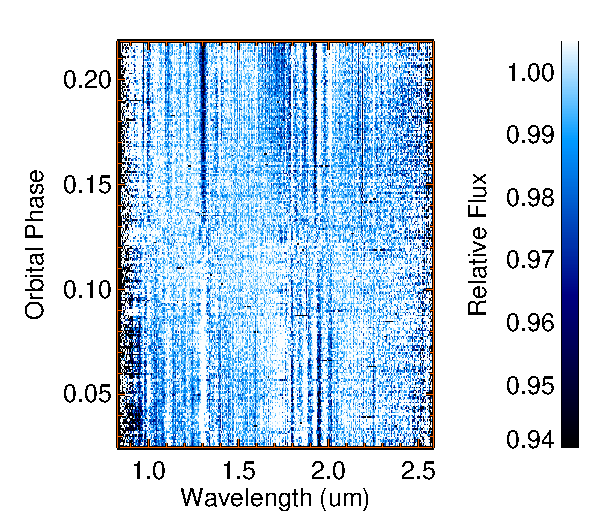
\includegraphics[width=0.5\textwidth]{specphot_0835_auto_noremovel.pdf}
	\label{fig:specphot0835autoS}
	}
\subfloat[2MASS J0835 - Manual shifting ]{
	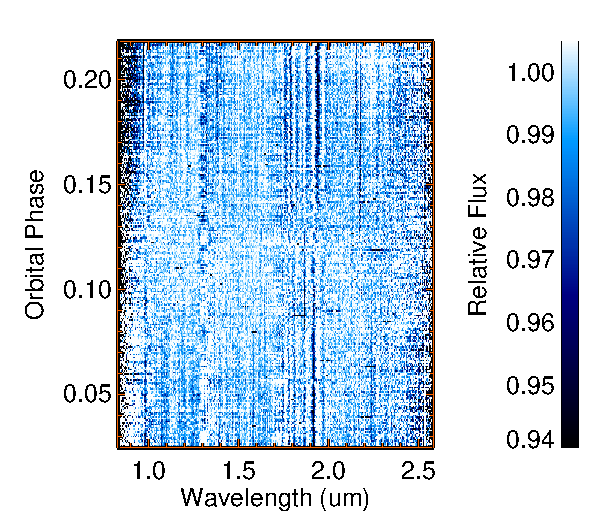
\includegraphics[width=0.5\textwidth]{specphot_0835_manual_noremovel.pdf}
	\label{fig:specphot0835manualS}
	}
	\caption{Dynamic spectra of {\sha} using automatic cross correlation wavelength shifting (left) and manual wavelength shifting(right).
	The manual method shows dramatically better systematics in these dynamic spectra which have no fits along columns to remove trends.}
	\label{fig:manualVsAutoShift0835}
	\vspace{0.1in}
\end{figure*} 


\begin{figure*}[!t]
\centering
\subfloat[2MASS J1821- Automatic Shifting]{
	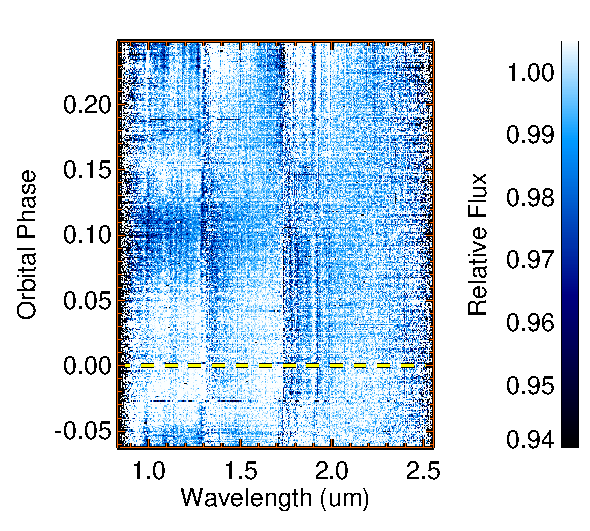
\includegraphics[width=0.5\textwidth]{specphot_1821_auto_noremovel.pdf}
	\label{fig:specphot1821autoS}
	}
\subfloat[2MASS J1821 - Manual shifting ]{
	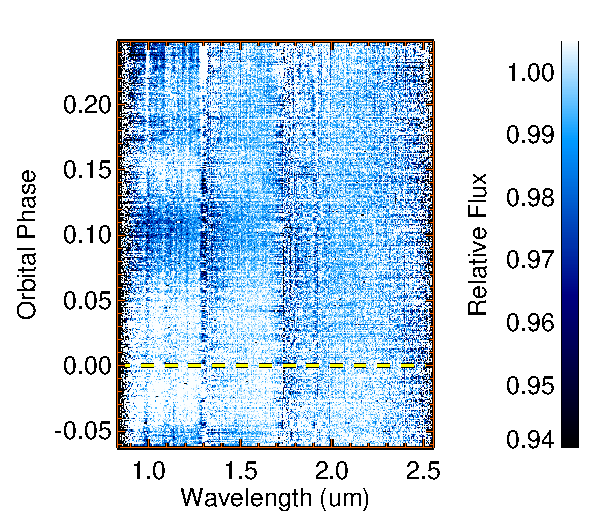
\includegraphics[width=0.5\textwidth]{specphot_1821_manual_noremovel.pdf}
	\label{fig:specphot1821manualS}
	}
	\caption{Dynamic spectra of {\shb} using automatic cross correlation wavelength shifting (left) and manual wavelength shifting(right).
	The manual method shows better systematics but higher frequency noise.}
	\label{fig:manualVsAutoShift1821}
	\vspace{0.1in}
\end{figure*} 

\clearpage
\pagebreak
\subsection{MCMC Time Series Fits - first try}

Fitting all light curves to \sha\ with MCMC methods and without the A$_1 >$ 0 prior results in more non-detections, but an unusual pattern to the spectra.
As with other MCMC fits, error bars are from photon and read noise, so they're likely under-estimated.

\begin{figure*}[!t]
\centering
\subfloat[2MASS J0835 - Manual Shifting]{
	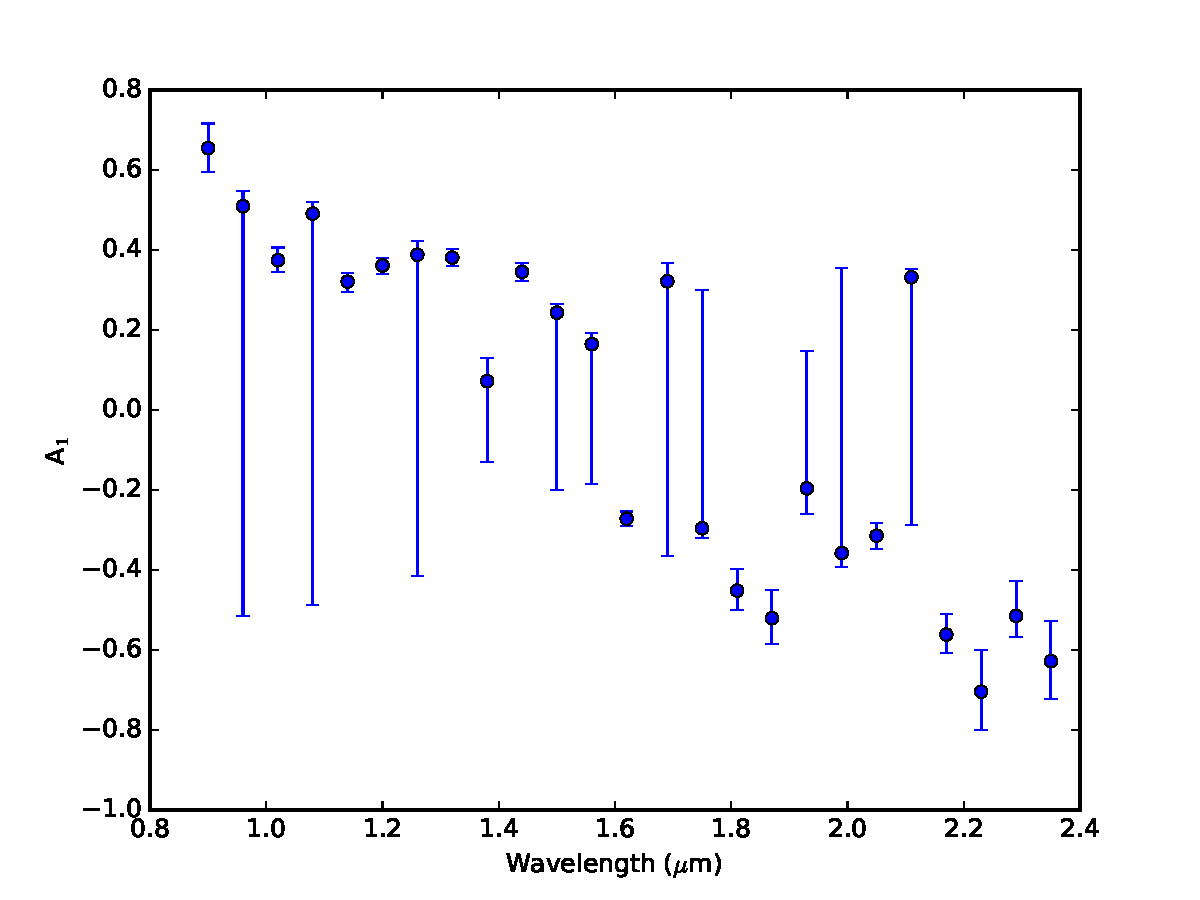
\includegraphics[width=0.5\textwidth]{mcmc_spectrum_2mass_0835.pdf}
	\label{fig:ampSpec0835ManualS}
	}
\subfloat[2MASS J1821 - Manual shifting ]{
	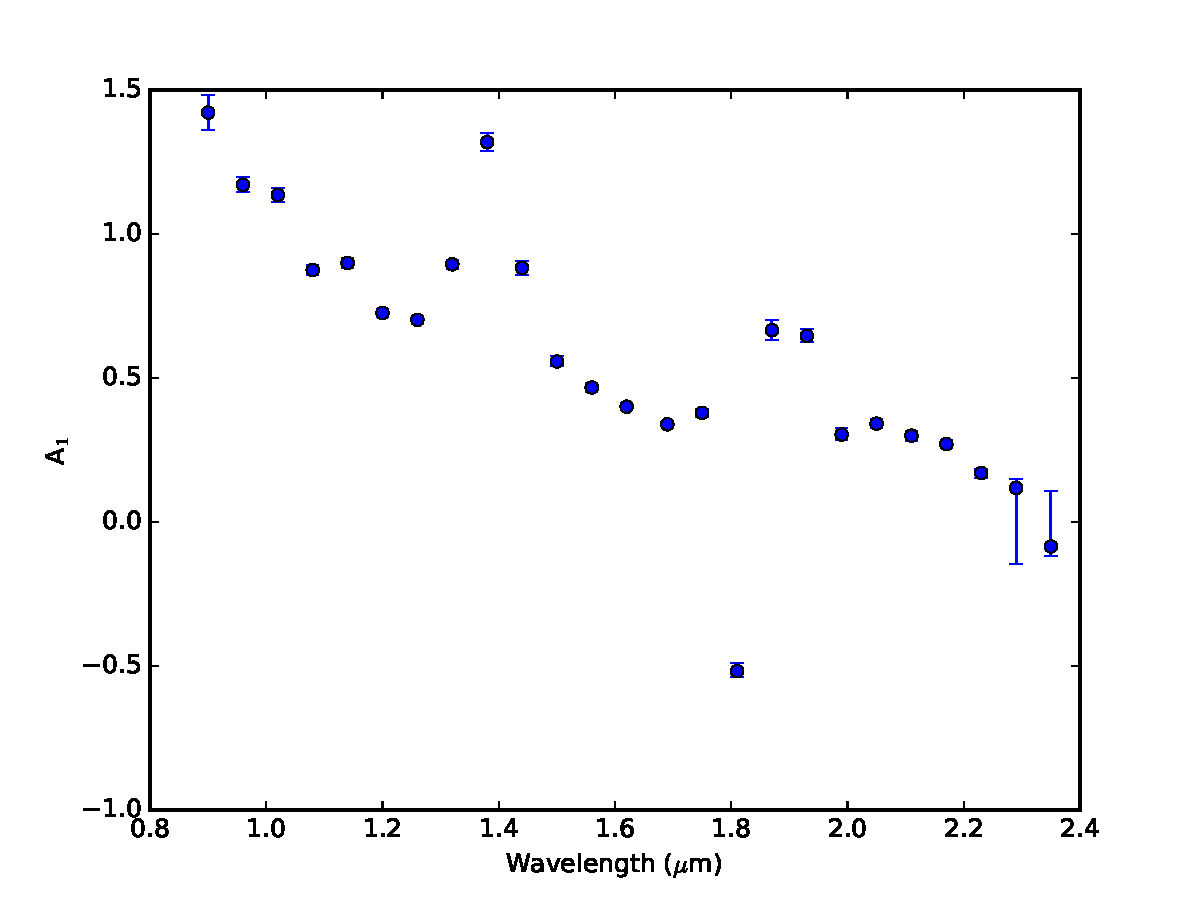
\includegraphics[width=0.5\textwidth]{mcmc_spectrum_2mass_1821.pdf}
	\label{fig:ampSpec1821ManualS}
	}
	\caption{Amplitude spectrum of {\sha} (left)  and {\shb} (right) using manual wavelength shifting, 1 cosine term fit and MCMC fitting with error bars from photon and read noise.}
	\label{fig:ampSpecManualS}
	\vspace{0.1in}
\end{figure*} 

\begin{figure*}[!t]
\centering
\subfloat[2MASS J0835 - 4$\times \sigma$]{
	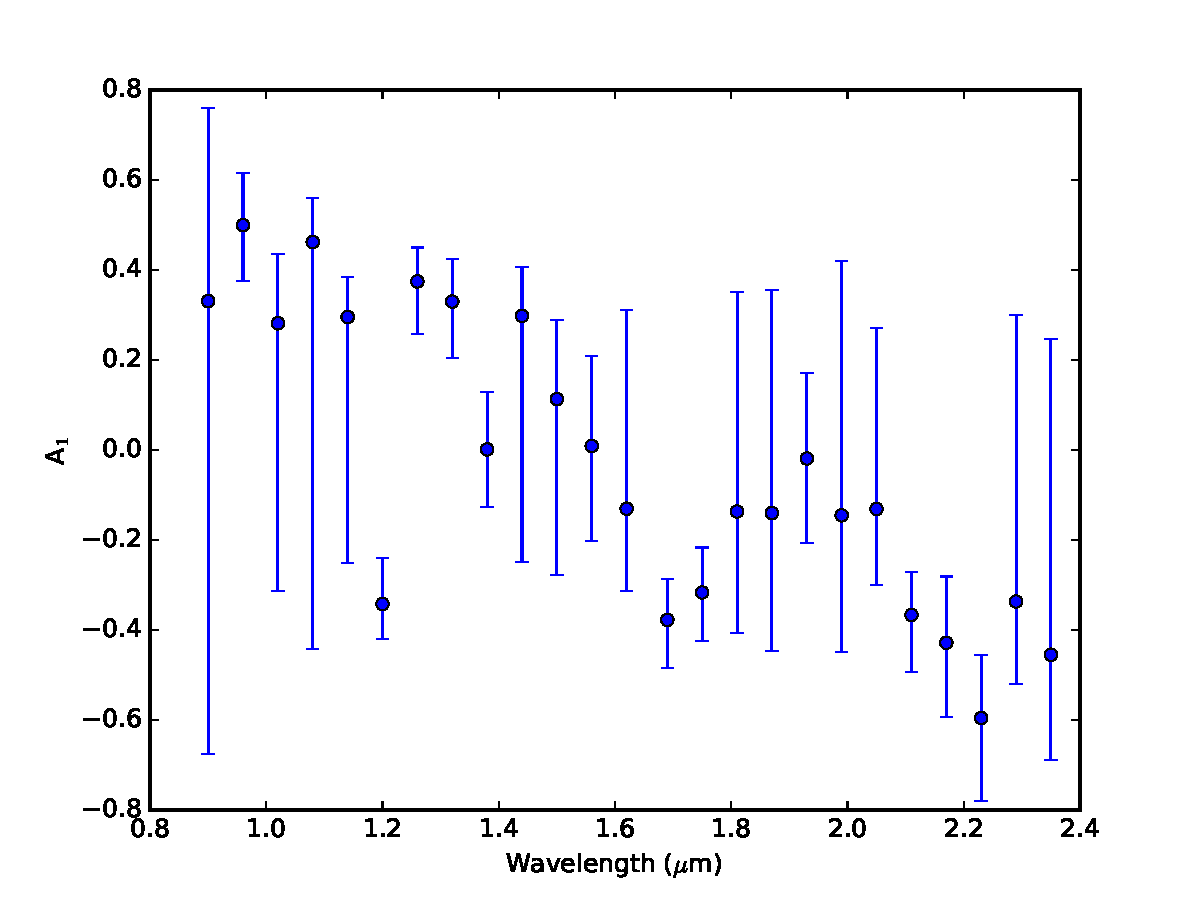
\includegraphics[width=0.5\textwidth]{mcmc_2mass_0835_spectrum_0400perc_err.pdf}
	\label{fig:ampSpec0835fourTimesErr}
	}
\subfloat[2MASS J1821 - 4$\times \sigma$ ]{
	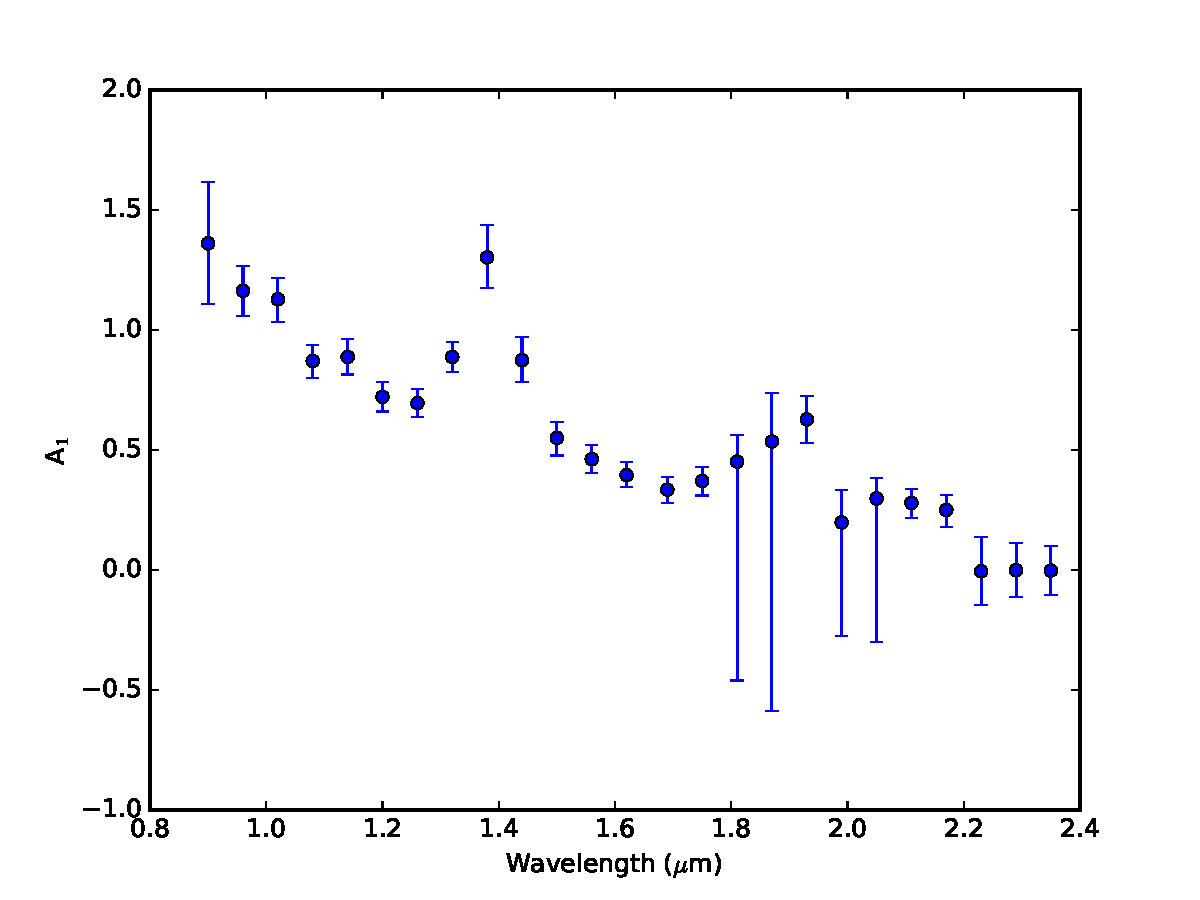
\includegraphics[width=0.5\textwidth]{mcmc_2mass_1821_spectrum_0400perc_err.pdf}
	\label{fig:ampSpec1821fourTimesErr}
	}
	\caption{As an experiment, I remade the amplitude spectra of Figure \ref{fig:ampSpecManualS} but scaled all error bars up by a factor of 4 for all points to account for some systematic errors. IE, Amplitude spectrum of {\sha} (left)  and {\shb} (right) using manual wavelength shifting, 1 cosine term fit and MCMC fitting with error bars from 4$\times$ photon and read noise.}
	\label{fig:ampSpecManualSfourTimesErr}
	\vspace{0.1in}
\end{figure*} 

\clearpage
\pagebreak
\subsection{MCMC Time Series Fits - second try}

As with my \texttt{IDL} code, I found that I had to impose a tight prior on the rotation period (I actually fixed it at the literature value of 4.1 hr) in order to avoid fitting the systematics at the telluric wavelengths.
When I do this, the MCMC code produces a very smooth amplitude spectrum for 2MASS 1821, as visible in Figure \ref{fig:ampSpecManualSTauRestrict}.
I experimented with the restriction that $3.8 < \tau < 4.0$ based on the multi-term Fourier series fits.
I used two different error scalings - 2.5 $\sigma$ and 4 $\sigma$.
2.5 $\sigma$ give the expected $\bar{\chi^2} \approx 1$, whereas 4 $\sigma$ gives around 0.4.


\begin{figure*}[!t]
\centering
\subfloat[2MASS J1821 - 2.5$\times \sigma$]{
	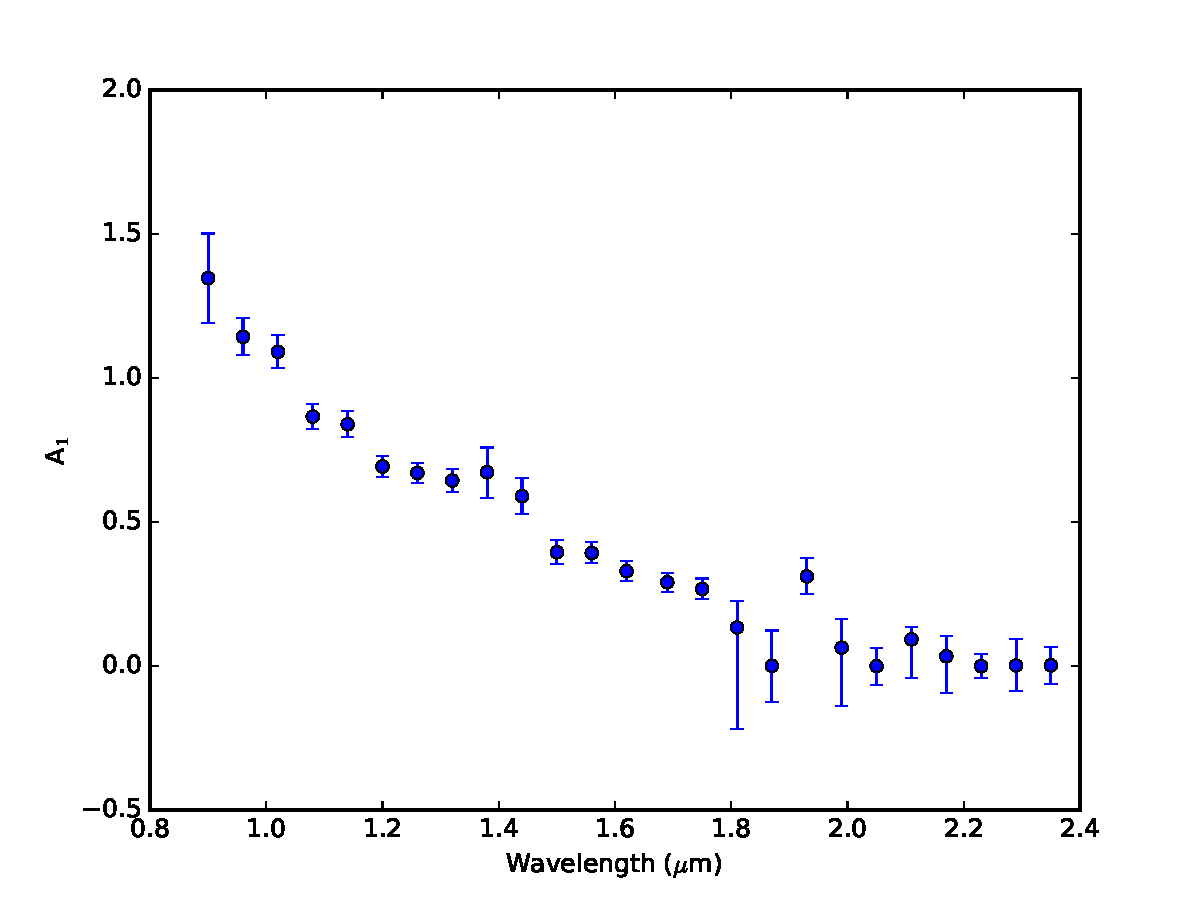
\includegraphics[width=0.5\textwidth]{2mass_1821_spectrum_0250perc_err_taurestrict.pdf}
	\label{fig:ampSpec1821times2p5ErrTauRest}
	}
\subfloat[2MASS J1821 - 4$\times \sigma$ ]{
	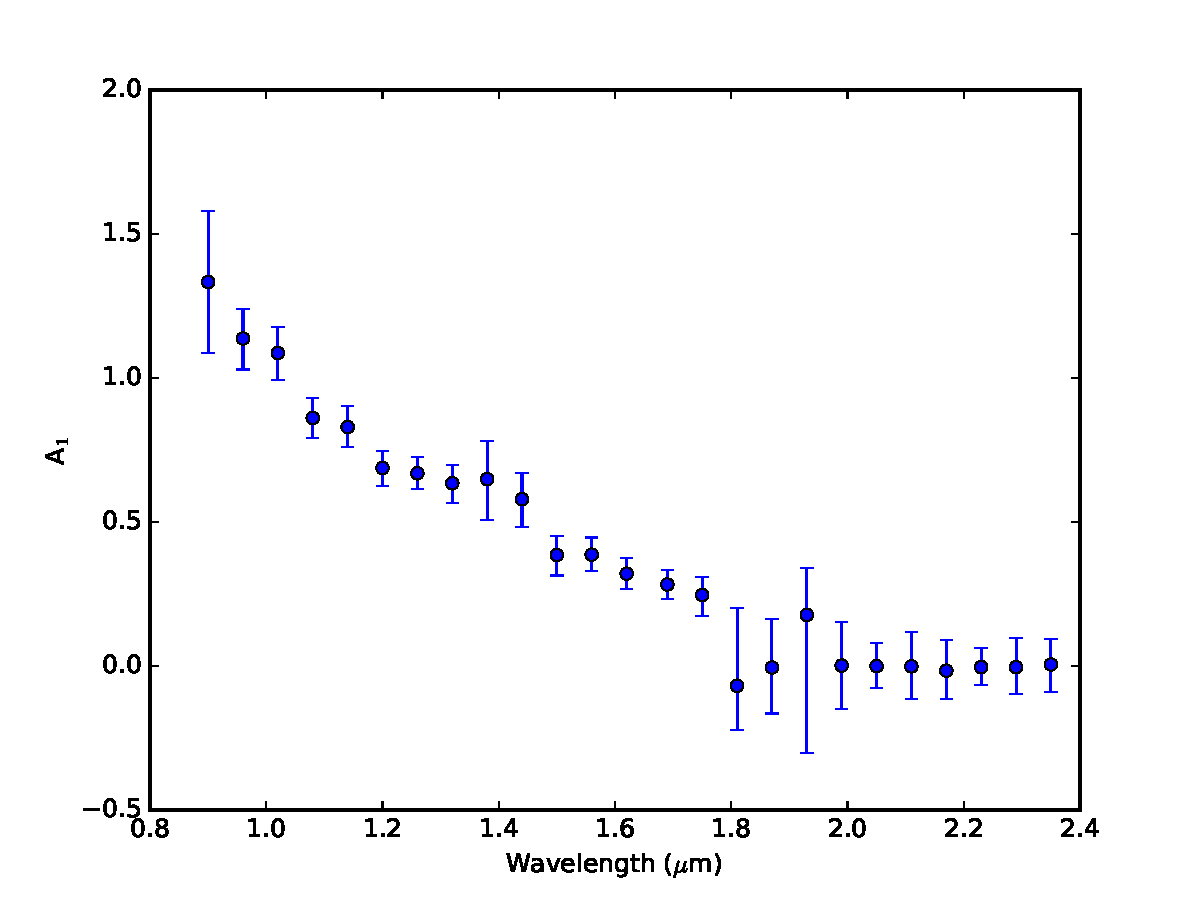
\includegraphics[width=0.5\textwidth]{2mass_1821_spectrum_0400perc_err_taurestrict.pdf}
	\label{fig:ampSpec1821fourTimesErrTauRest}
	}
	\caption{Restricting the $\tau$ parameter to, $3.8 < \tau < 4.0$ significantly reduces the long term quadratic terms' contribution to the sinusoidal fit. In this case, there were MCMC fits for \shb, one with error bars scaled by 2.5$\sigma$ and the other by 4.0$\sigma$.}
	\label{fig:ampSpecManualSTauRestrict}
	\vspace{0.1in}
\end{figure*} 

As with \shb\ I imposed a tight prior on $\tau$ such that $3.0 < \tau < 3.2$ for \sha. This now gives an average amplitude of zero -- see Figure \ref{fig:ampSpec0835TauRestrict}.

\begin{figure*}[!t]
\centering
\subfloat[2MASS J0835 - 2.5$\times \sigma$]{
	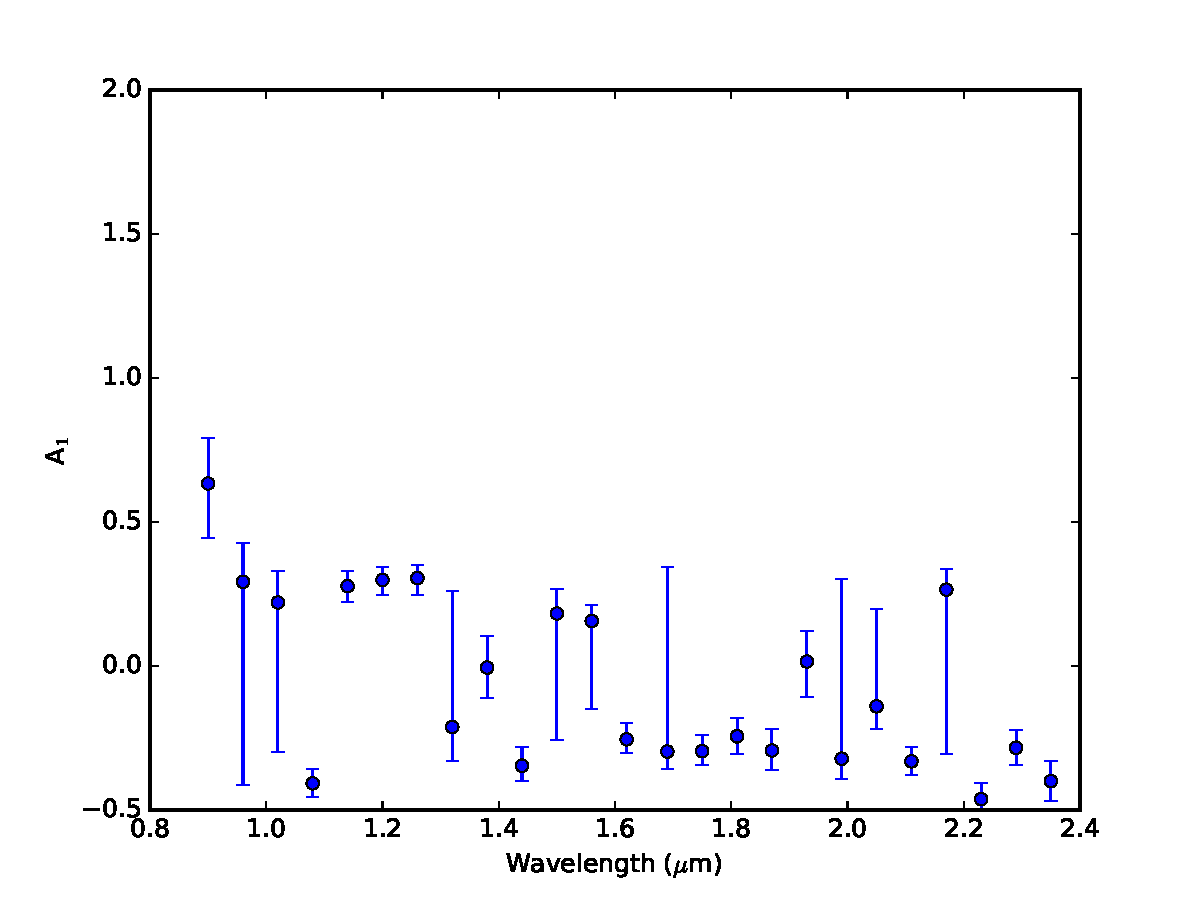
\includegraphics[width=0.5\textwidth]{2mass_0835_spectrum_0250perc_err_taurestrict.pdf}
	\label{fig:ampSpec0835times2p5ErrTauRest}
	}
\subfloat[2MASS J0835 - 4$\times \sigma$ ]{
	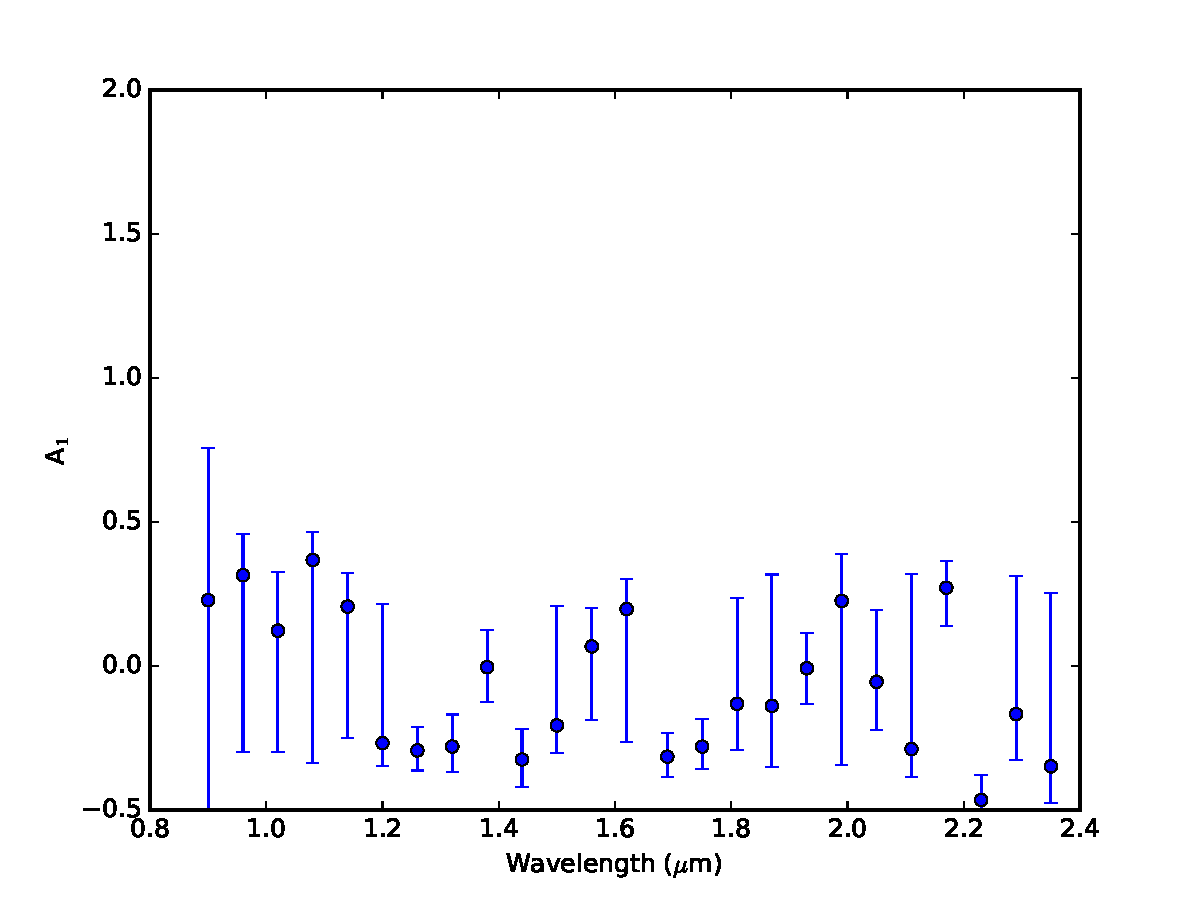
\includegraphics[width=0.5\textwidth]{2mass_0835_spectrum_0400perc_err_taurestrict.pdf}
	\label{fig:ampSpec0835fourTimesErrTauRest}
	}
	\caption{Restricting the $\tau$ parameter to $3.0 < \tau < 3.2$ results in a spectrum that is on average near 0\% amplitude for \sha. We show the amplitude spectra for error bars scaled by 2.5$\sigma$ and 4.0$\sigma$.}
	\label{fig:ampSpec0835TauRestrict}
	\vspace{0.1in}
\end{figure*} 

One thing to check is the time offset parameter as a function of wavelength.
AB noticed a trend in this $t_1$ parameter, but didn't have error bars fully incorporated.
I'm finding the trend is marginal when using 4$\sigma$ noise scaling.

\begin{figure*}[!t]
\centering
\subfloat[2MASS J0835 - 4$\times \sigma$]{
	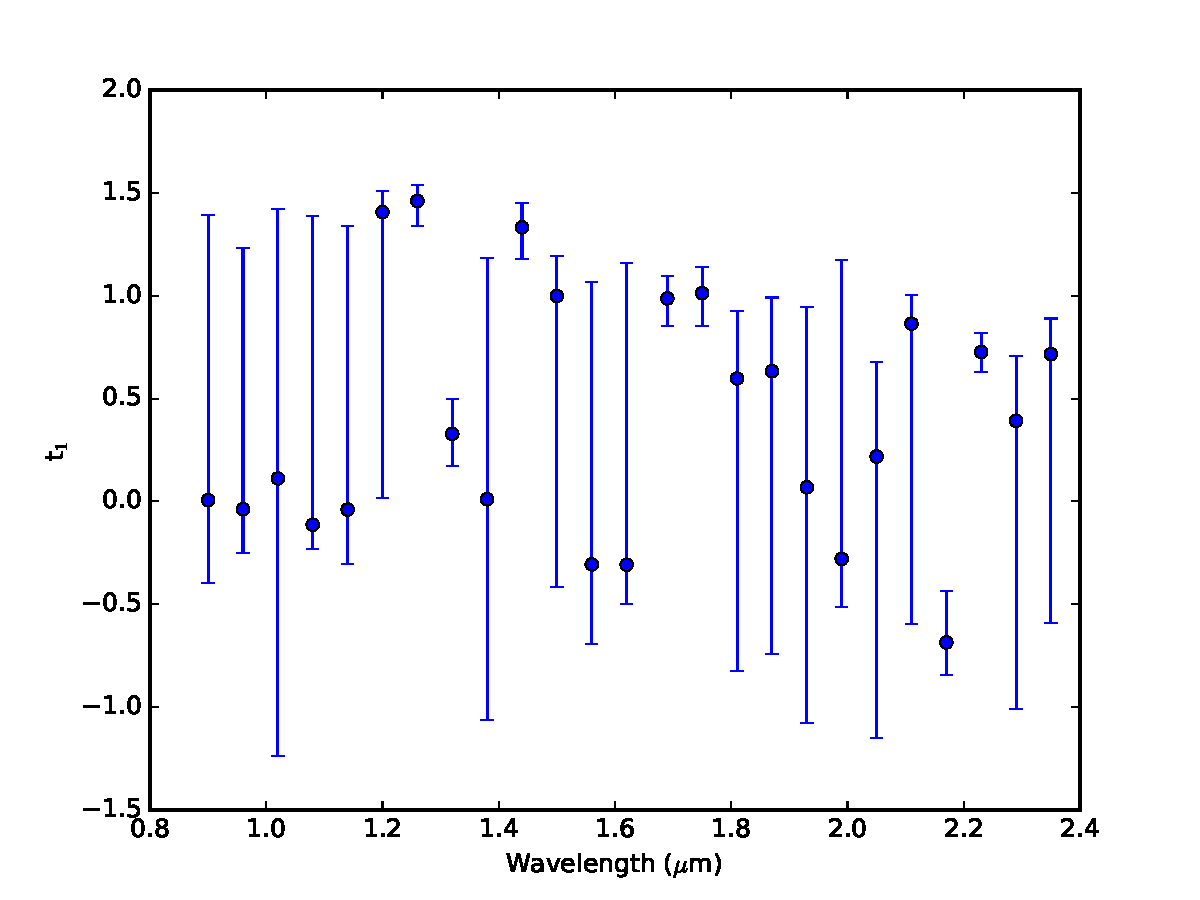
\includegraphics[width=0.5\textwidth]{2mass_0835_t_1_spectrum_0400perc_err_taurestrict.pdf}
	\label{fig:t1Spec0835TauRest}
	}
\subfloat[2MASS J1821 - 4$\times \sigma$ ]{
	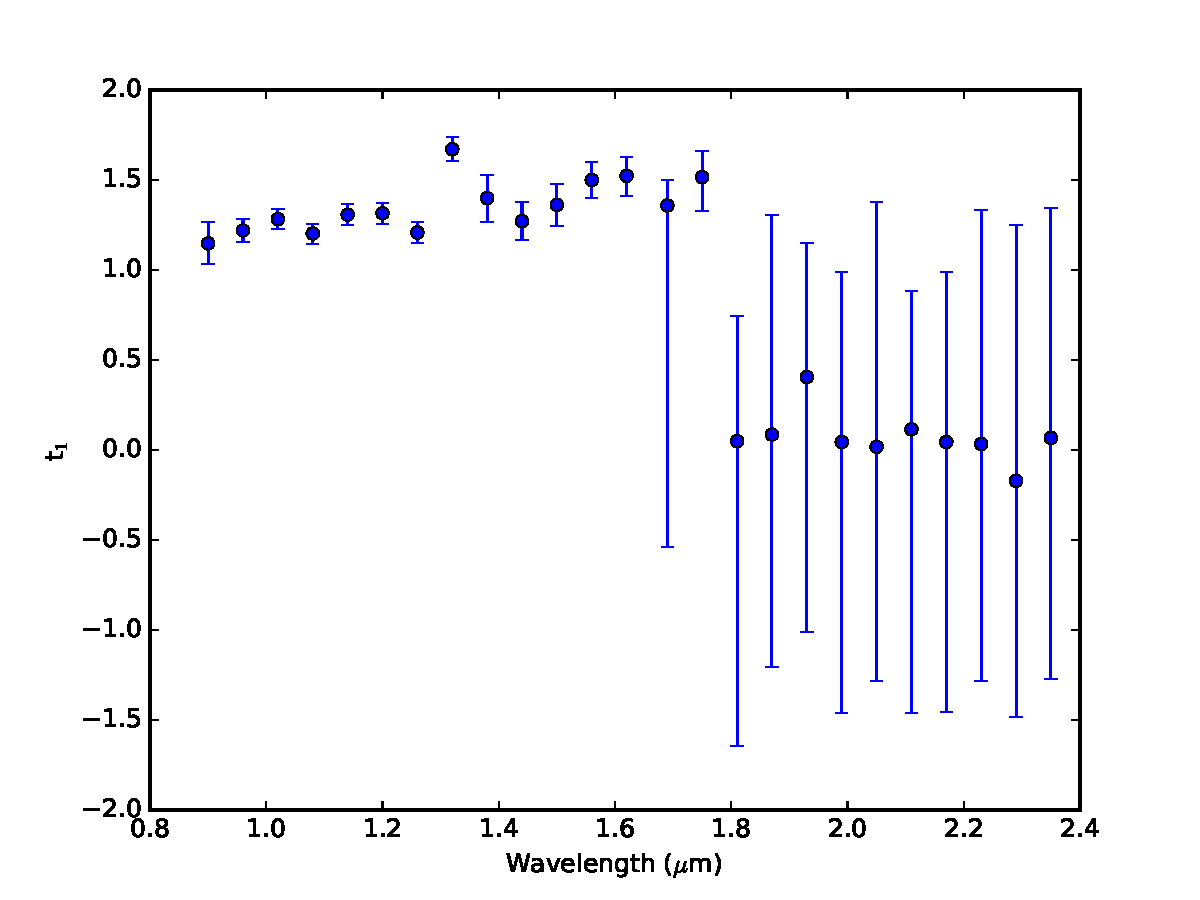
\includegraphics[width=0.5\textwidth]{2mass_1821_t_1_spectrum_0400perc_err_taurestrict.pdf}
	\label{fig:t1Spec1821TauRest}
	}
	\caption{Searching for trends in the $t_1$ parameter as a function of wavelength. The possible upward trend is marginal for \shb\ when using the 4$\sigma$ scaling of error bars. In these cases, we have restricted the $\tau$ parameter with priors to $3.0 < \tau < 3.2$ and $3.8 < \tau < 4.0$ for \sha\ and \shb\ respectively.}
	\label{fig:t1SpecTauRestrict}
	\vspace{0.1in}
\end{figure*} 

\begin{figure*}[!t]
\centering
\subfloat[2MASS J0835 - 4$\times \sigma$]{
	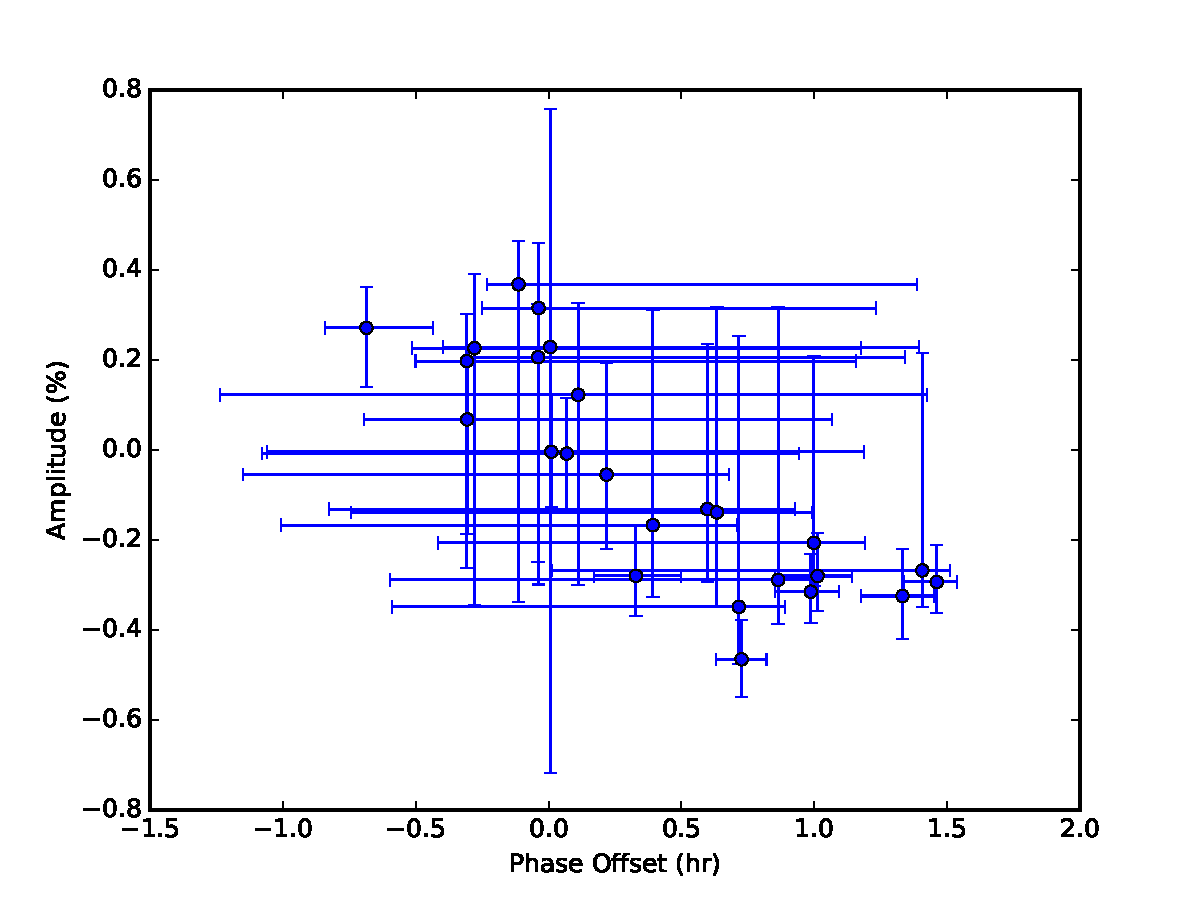
\includegraphics[width=0.5\textwidth]{2mass_0835_t1_vs_A1_0400perc_err_taurestrict.pdf}
	\label{fig:t1vsA1Spec0835}
	}
\subfloat[2MASS J1821 - 4$\times \sigma$ ]{
	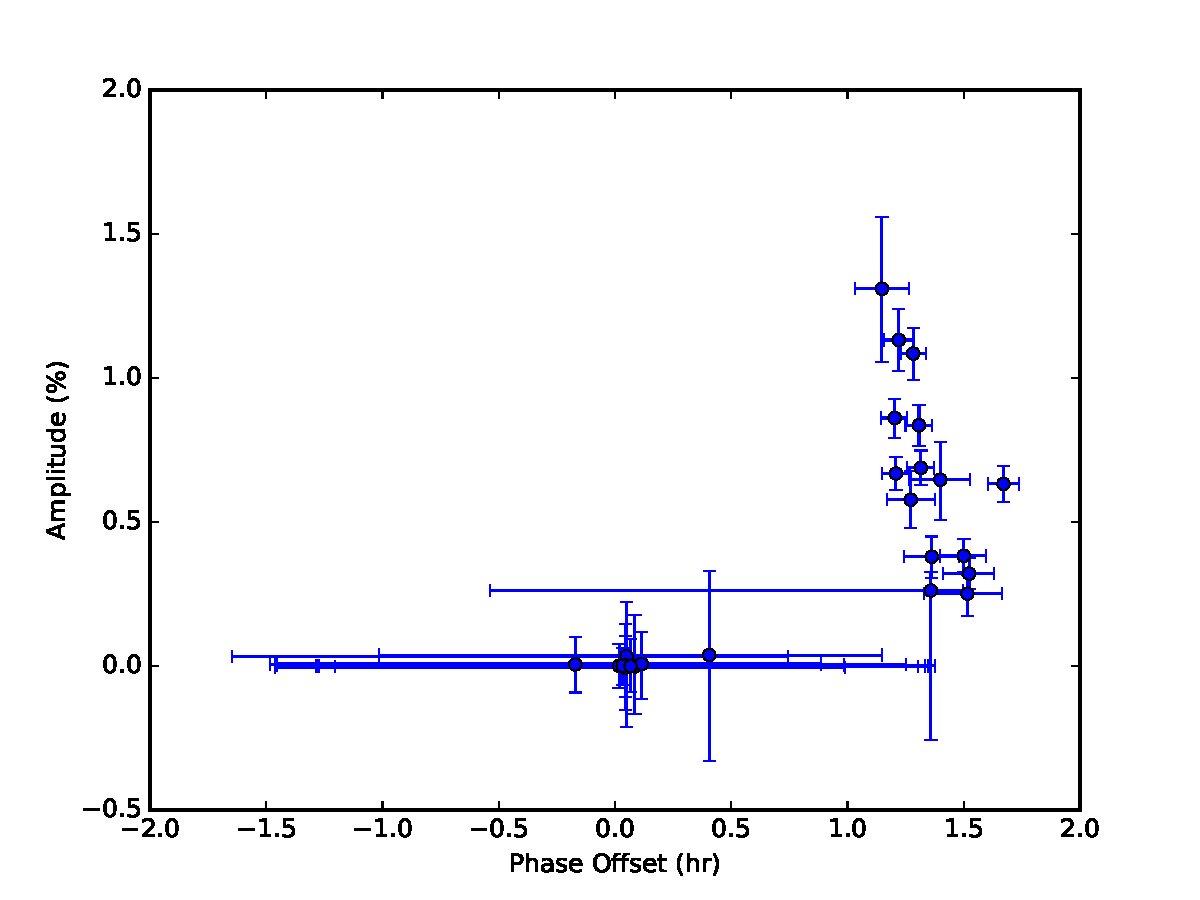
\includegraphics[width=0.5\textwidth]{2mass_1821_t1_vs_A1_0400perc_err_taurestrict.pdf}
	\label{fig:t1vsA1Spec1821}
	}
	\caption{Searching for trends in the $t_1$ parameter as a function of Amplitude ($A_1$). No clear trend arises in these correlation plots. As with Figure \ref{fig:t1SpecTauRestrict}, we have used 4$\sigma$ scaling of error bars and restricted the $\tau$ parameter with priors to $3.0 < \tau < 3.2$ and $3.8 < \tau < 4.0$ for \sha\ and \shb\ respectively.}
	\label{fig:t1vsA1SpecTest}
	\vspace{0.1in}
\end{figure*} 


\clearpage
\pagebreak
\subsection{Mie scattering MCMC}

My old Mie scattering code was in IDL and would be more work to incorporate into MCMC fitting, so I found python package \texttt{miescatter} and did a comparison with my IDL code.

\begin{figure}
\begin{centering}
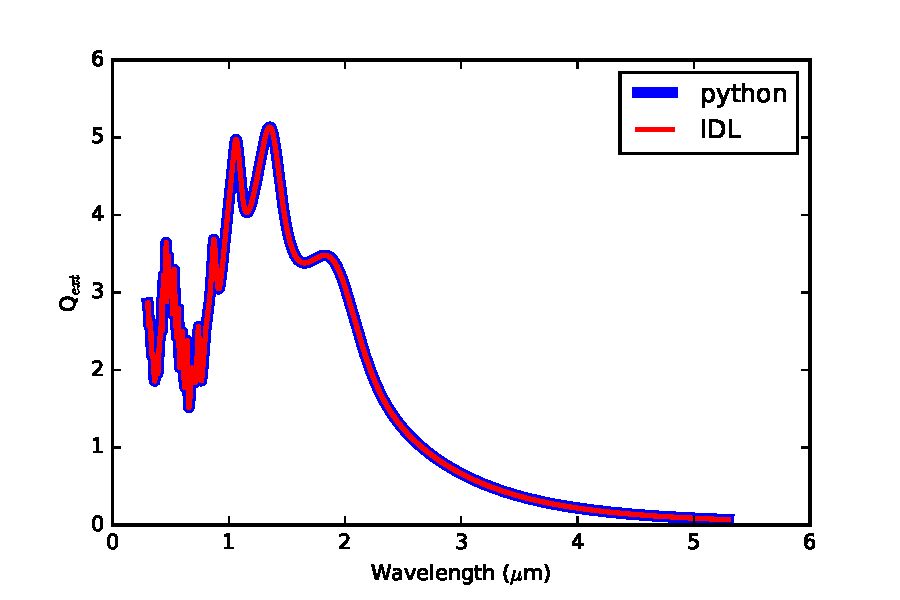
\includegraphics[width=0.5\textwidth]{python_vs_IDL_example.pdf}
\caption{Example Mie scattering extinction cross sections $Q_{ext}$ for a spherical particle with a radius of 0.5~$\mu$m and a complex index of refraction of n=1.825 - 0.001 $i$. The IDL and python code's are in excellent agreement.}\label{fig:IDLvsPython}
\end{centering}
\end{figure}

I did an initial MCMC fit where I plugged in these same index of refraction (n=1.825 - 0.001 $i$ for all wavelengths) and fit the spectrum that I found in IDL.
The best fit matches the data well with a $\bar{\chi^2}$ of 1.3, visible in Figure \ref{fig:mcmcMieBest1particle}.
However, there are many solutions at different resonances in the Mie extinction curve visible in Figure \ref{fig:mcmcMieCorner1particle}.
A better way to handle this is a log-normal distribution of particles as in \citet{2016ApJ...826..156S}.

\begin{figure*}[!t]
\centering
\subfloat[Single Particle Best fit for \shb]{
	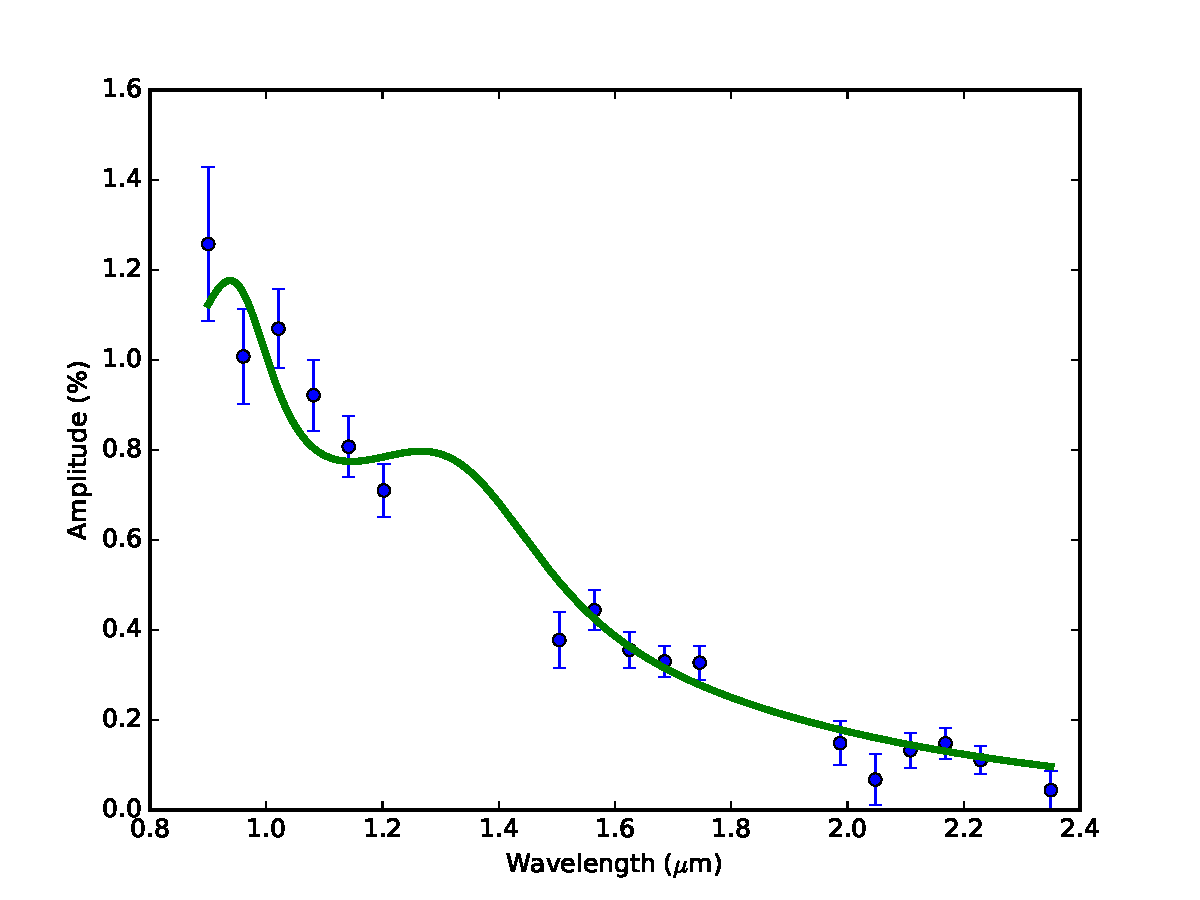
\includegraphics[width=0.5\textwidth]{best_fit_single_particle_mie.pdf}
	\label{fig:mcmcMieBest1particle}
	}
\subfloat[Single Particle Posterios for \shb]{
	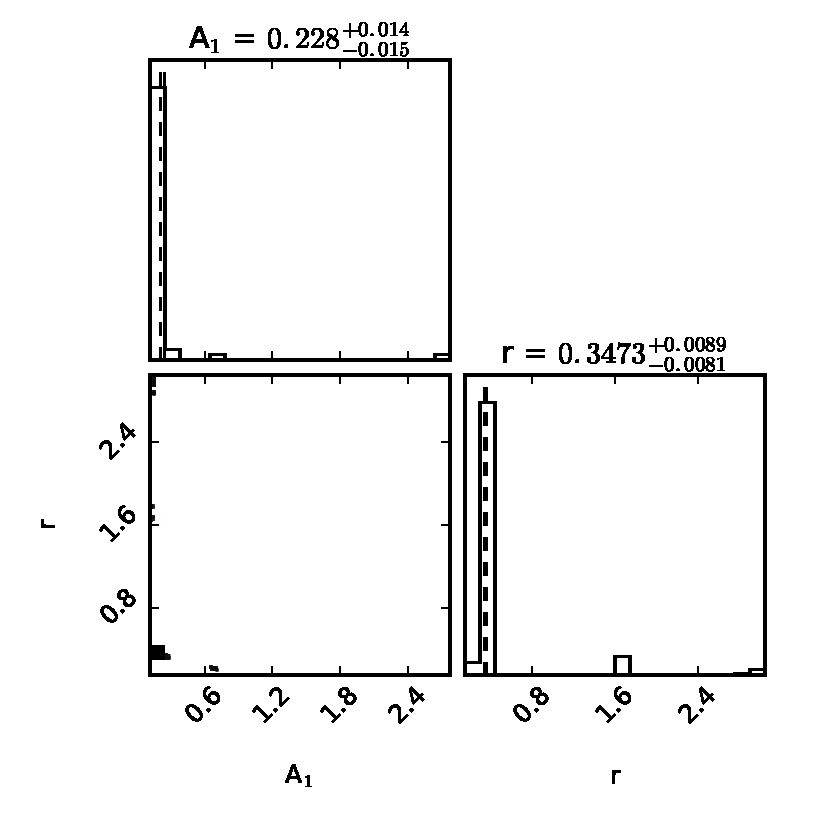
\includegraphics[width=0.5\textwidth]{corner_single_particle_mie.pdf}
	\label{fig:mcmcMieCorner1particle}
	}
	\caption{An initial fit to the amplitude spectrum when using a single particle.
	The best fit nicely matches the data but has multiple solutions at the Mie scattering resonances.}
	\label{fig:mcmcMieCorner1particle}
	\vspace{0.1in}
\end{figure*} 

I manually created a log-normal distribution of particles in Python and added up their cross sections weighted by number of particles.
This process is slow, so I calculated it once and found  a 15th order polynomial fit to $Q_{ext}$ and evaluated this in the model.
The resulting MCMC distribution is shown in Figure \ref{fig:mcmcMieCornerLogNorm}.

\begin{figure*}[!t]
\centering
\subfloat[Log-Normal Best fit for \shb]{
	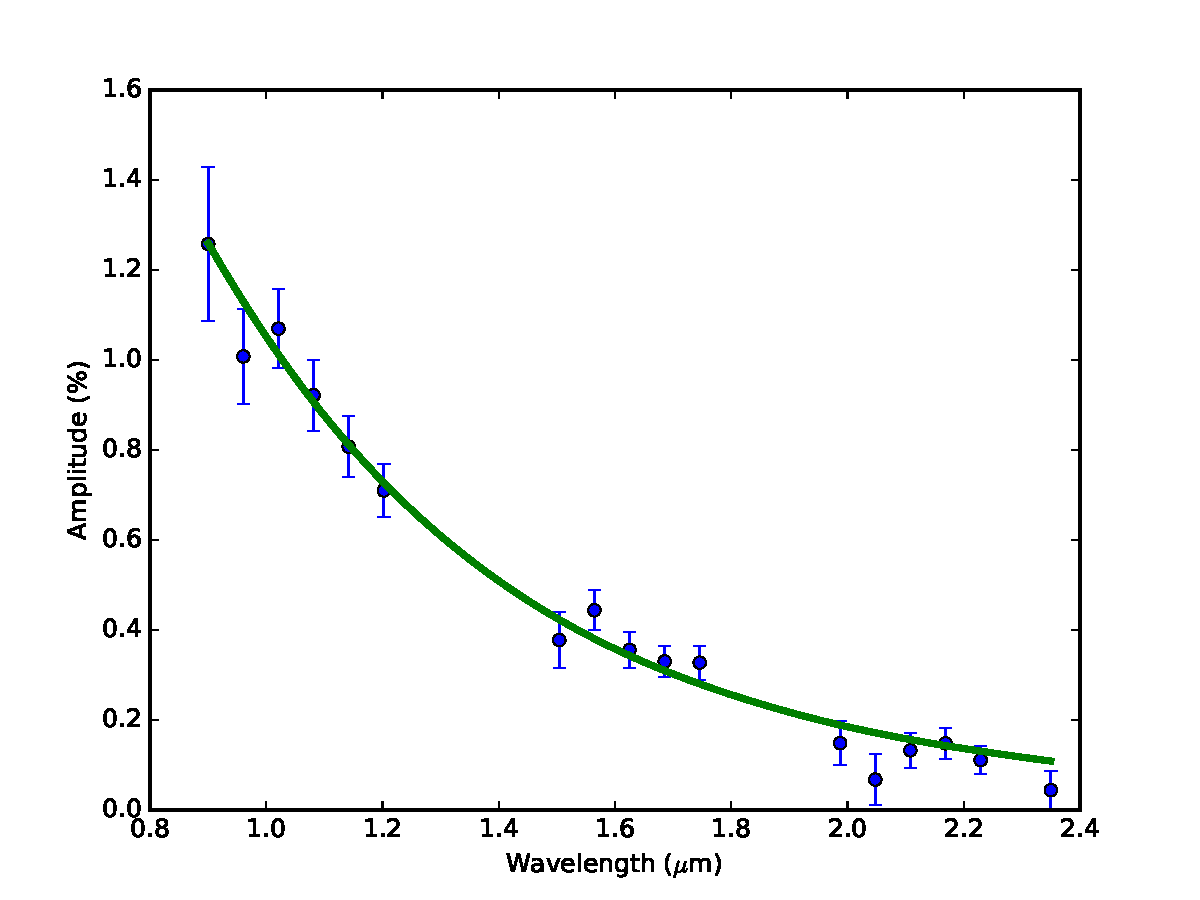
\includegraphics[width=0.5\textwidth]{best_fit_lognormal_mie.pdf}
	\label{fig:mcmcMieBestLogNorm}
	}
\subfloat[Log-Normal Posteriors for \shb]{
	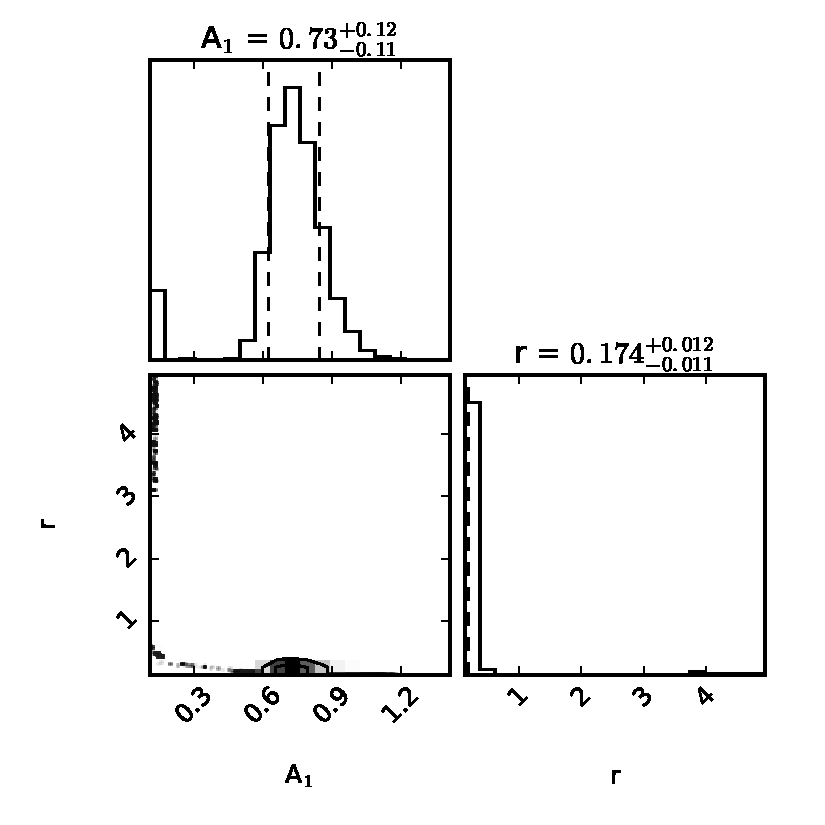
\includegraphics[width=0.5\textwidth]{corner_lognormal_mie.pdf}
	\label{fig:mcmcMieCornerLogNorm}
	}
	\caption{An initial fit to the amplitude spectrum when using a log-normal size distribution with a $\sigma=0.5$.
	Again, there are a few ``walkers'' that stay at large radii.}
	\label{fig:mcmcMieCornerLogNorm}
	\vspace{0.1in}
\end{figure*} 

On closer inspection, I see that there is a local minimum for large particle radii where the $\chi^2$ begins to increase from 3~$\mu$m to 2$\mu$m.
This is illustrated in Figure \ref{fig:localMinLargeRadii}.
\begin{figure}
\begin{centering}
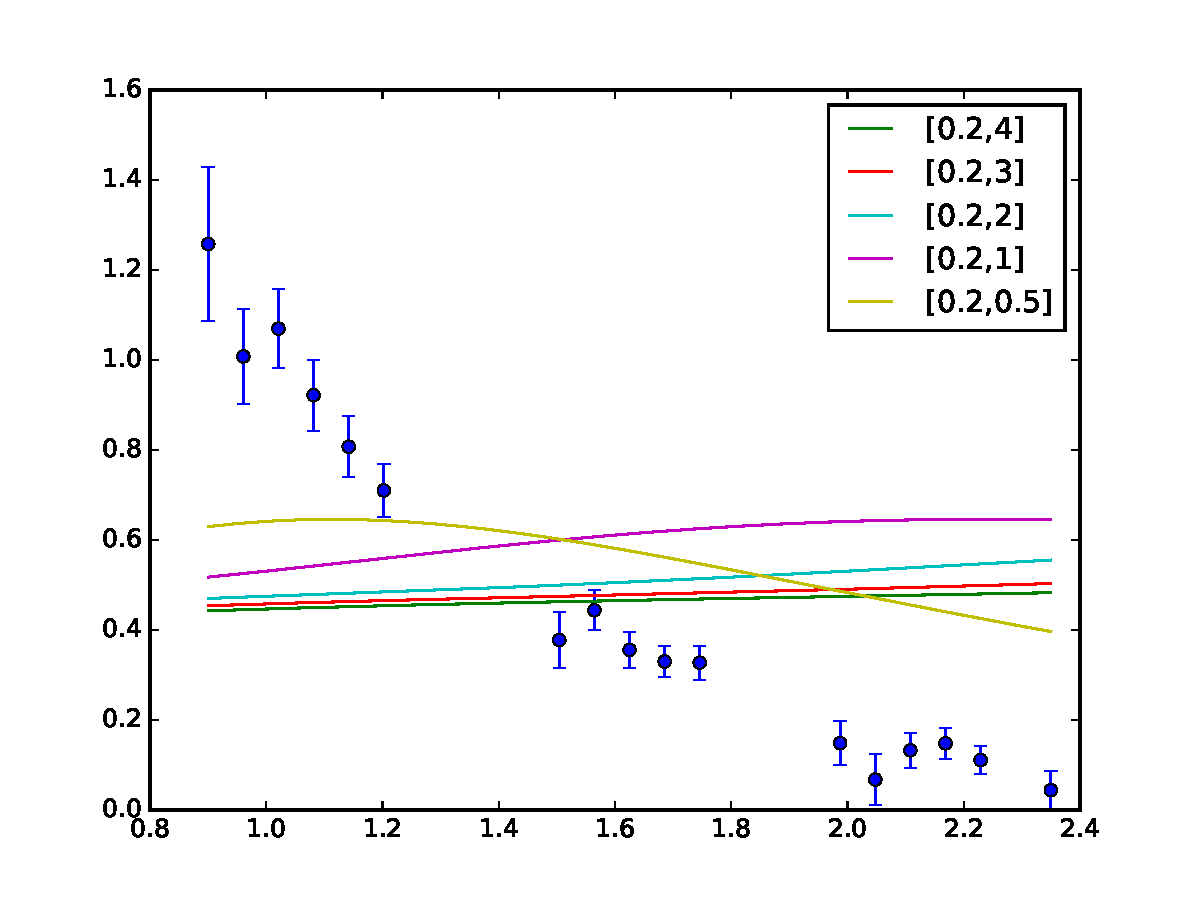
\includegraphics[width=0.5\textwidth]{local_min_illustration.pdf}
\caption{A set of example Mie scattering models for example parameters for the Amplitude offset and median particle radius written as [A,r]. The model at 2~$\mu$m is slightly worse than at 3~$\mu$m, so it traps a few walkers in the MCMC run.}\label{fig:localMinLargeRadii}
\end{centering}
\end{figure}

When I discard walkers with very low likelihood, as done in CHIMERA, the local minima are not included since their so low probability.
The resulting MCMC run is shown in Figure \ref{fig:localMinExcludeCorner}.

\begin{figure}
\begin{centering}
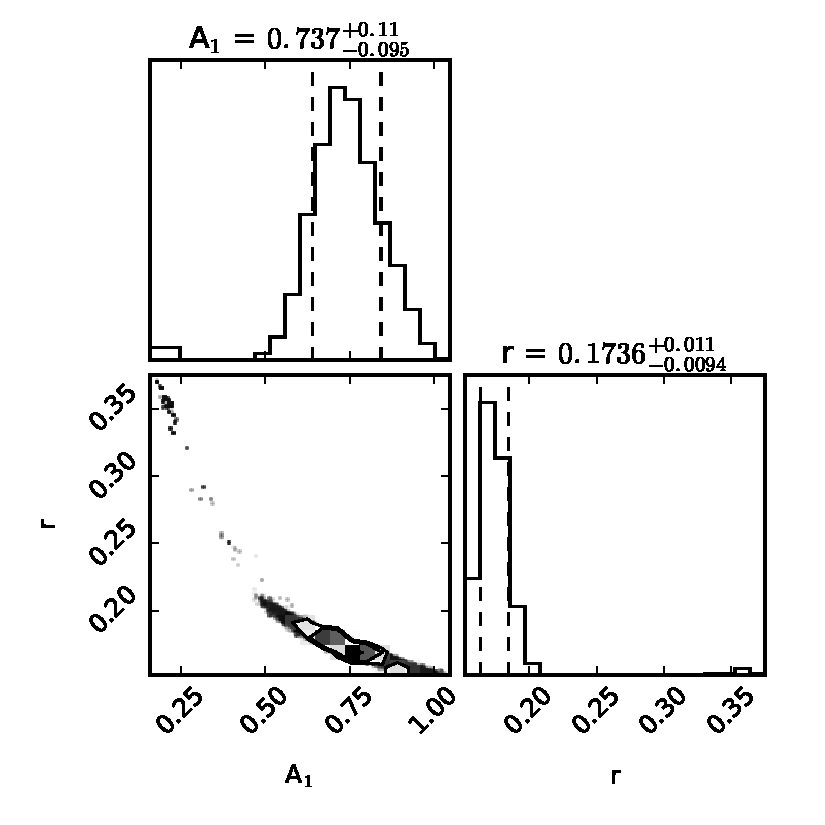
\includegraphics[width=0.5\textwidth]{corner_lognormal_mie_no_lmin.pdf}
\caption{MCMC fit when discarding points with a $\chi^2$ more than 5 times the minimum to exclude walkers that were trapped at local minima.}\label{fig:localMinExcludeCorner}
\end{centering}
\end{figure}

\clearpage
\pagebreak
\subsection{MORIS Data}

I made a time series of the MORIS $i$ band photometry to see if it would help with the spectrum fit.
The SNR is so low that's it hard to see any clear pattern.
However, the photometry can put upper limits to the spectrum, as seen in Figure \ref{fig:spectrum1821WMoris}.

\begin{figure*}[!t]
\centering
\subfloat[MORIS $i$ Band Photometry for \shb]{
	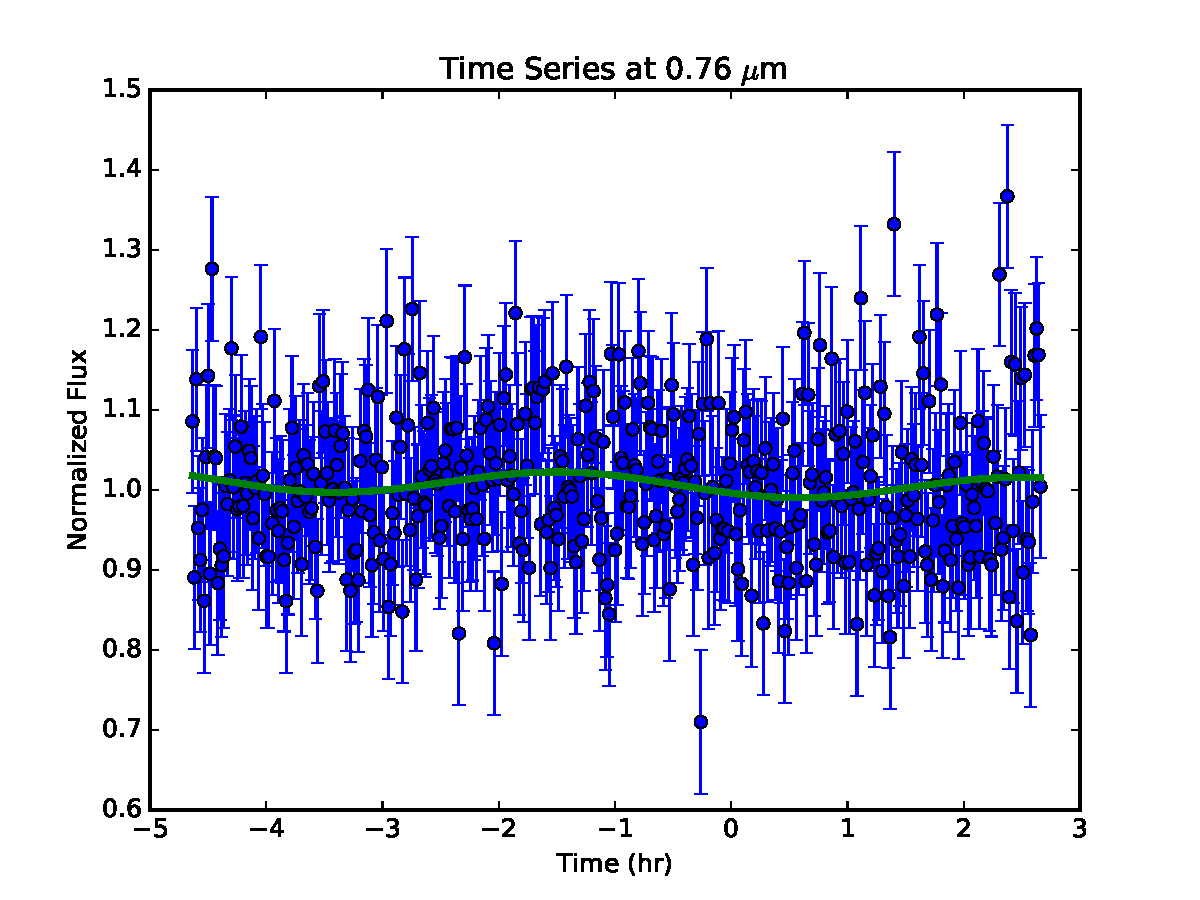
\includegraphics[width=0.5\textwidth]{2mass_1821_moris_tser_best_fit.pdf}
	\label{fig:morisTSerBestFit}
	}
\subfloat[Amplitude spectrum for \shb\ when adding MORIS photometry]{
	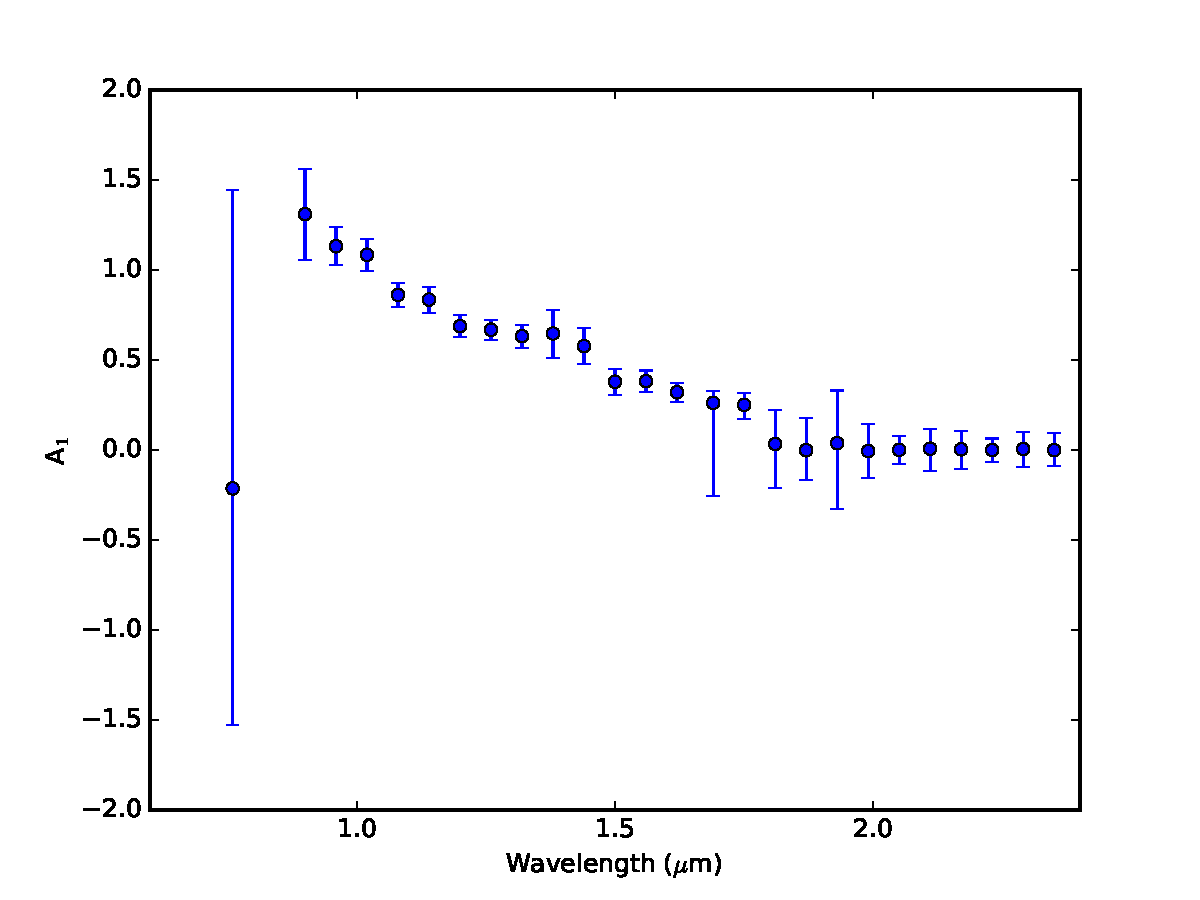
\includegraphics[width=0.5\textwidth]{2mass_1821_a1_spec_w_moris.pdf}
	\label{fig:spectrum1821WMoris}
	}
	\caption{MORIS photometry can put an upper limit on the short wavelength end of the spectrum spectrum.}
	\label{fig:morisPhotometryAndSpec}
\end{figure*} 


\clearpage
\section{Airmass Correlation}
One thing to check is that the U shaped light curves near the telluric water bands are correlated to airmass.
As I start, I took a time series at 1.26~$\mu$m to remove find a trend-line for brown dwarf modulations and any other tends.
This is shown in Figure \ref{fig:1p26umFluxTrendFit}.
I then remove this polynomial trend from the 1.38~$\mu$m time series to remove the brown dwarf oscillations from it.
The residual light curve has a U shape similar to the airmass trend shown in Figure \ref{fig:1p38residAndAirmass}.
A direct correlation plot is shown in Figure \ref{fig:residAirmass1p38corr}.

\begin{figure*}[!t]
\centering
\subfloat[Flux at 1.26~$\mu$m for the Trend-line]{
	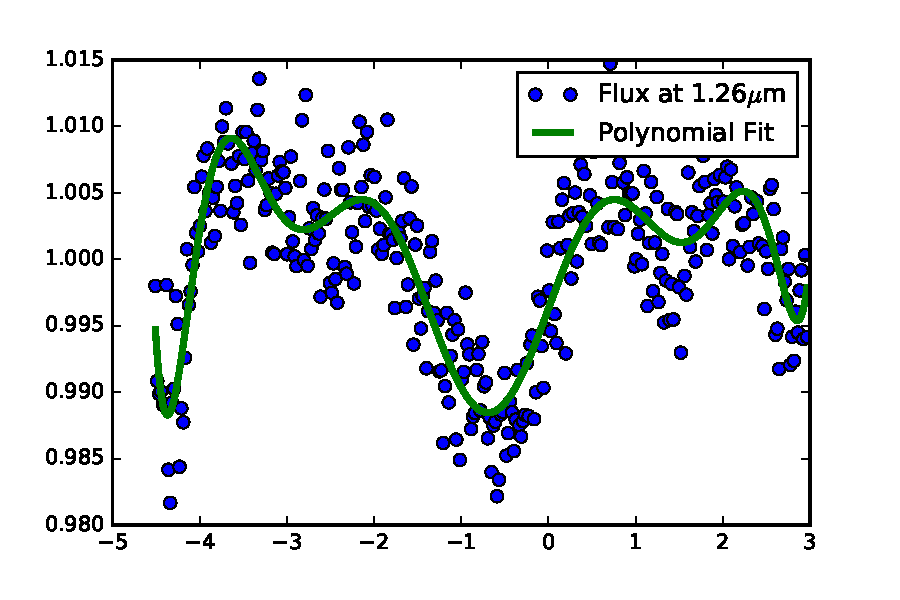
\includegraphics[width=0.5\textwidth]{images/airmass/trendline_1p26um.pdf}
	\label{fig:1p26umFluxTrendFit}
	}
\subfloat[Flux at 1.38~$\mu$m and Airmass]{
	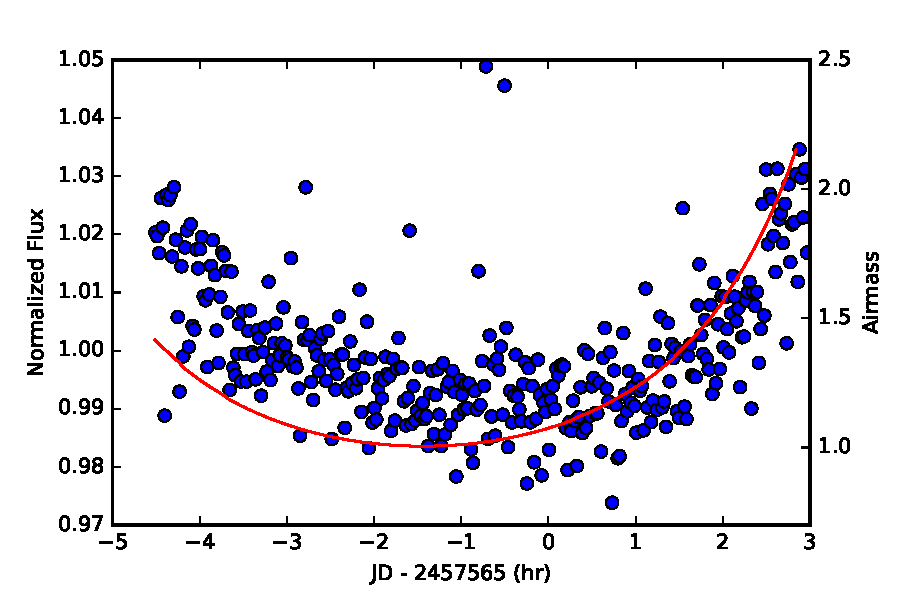
\includegraphics[width=0.5\textwidth]{images/airmass/airmass_1p38um_resid_simult.pdf}
	\label{fig:1p38residAndAirmass}
	}
	\caption{In order to investigate correlations with airmass at 1.38~$\mu$m, I first fit the 1.26~$\mu$m time series with a 10th order polynomial fit.
	I then use the polynomial fit to remove most of the brown dwarf related oscillations in the time series at 1.38$\mu$m. The residuals show a U shape similar to the airmass table.}
	\label{fig:airmassTimeSer1p38}
\end{figure*} 


\begin{figure}
\begin{centering}
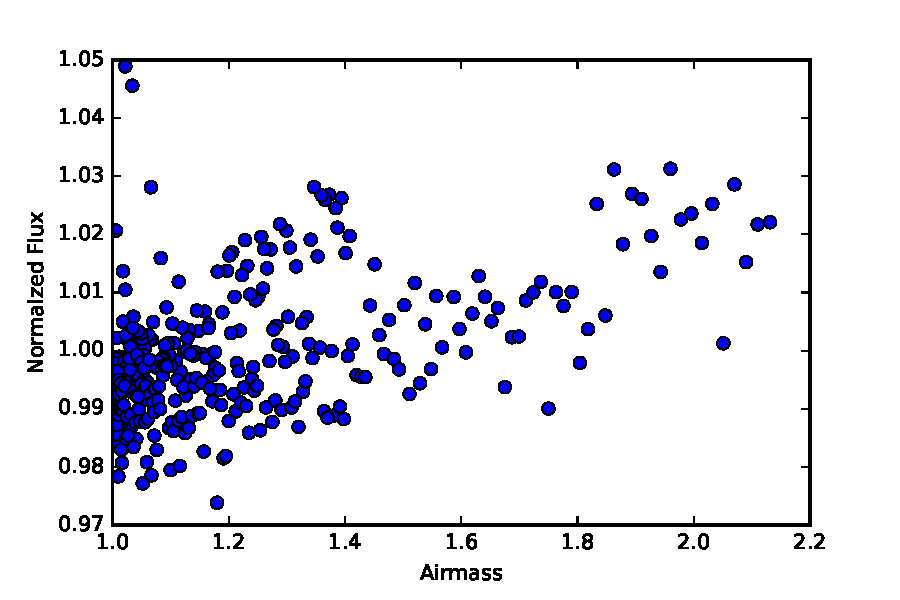
\includegraphics[width=0.5\textwidth]{images/airmass/airmass_flux_correlation.pdf}
\caption{Time series at 1.38$\mu$m as a function of airmass, where the brown dwarf oscillations are mostly removed as described in Figure \ref{fig:airmassTimeSer1p38}.}\label{fig:residAirmass1p38corr}
\end{centering}
\end{figure}

\clearpage
\section{Original Plots for reference}
\begin{figure*}
\centering
\subfloat[2MASS J0835 - \colorbox{red}{fit might need more work} ]{
	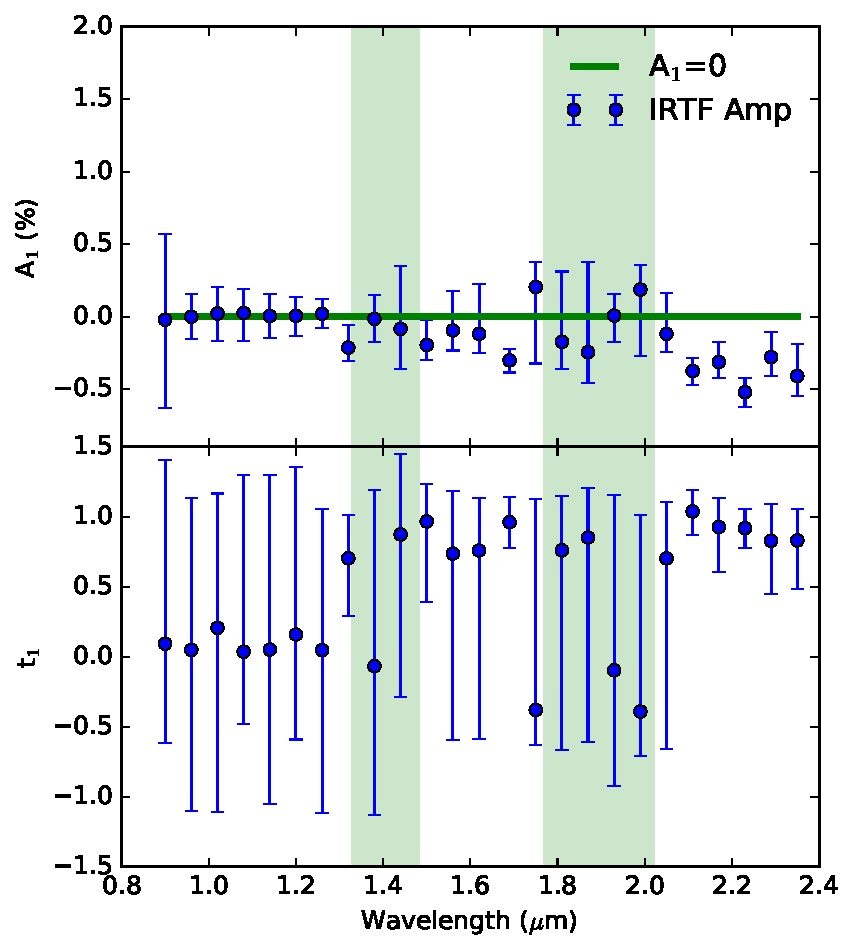
\includegraphics[width=0.5\textwidth]{amp_vs_wavl_j0835.pdf}
	\label{fig:ampspec0835}
	}
\subfloat[2MASS J1821]{
	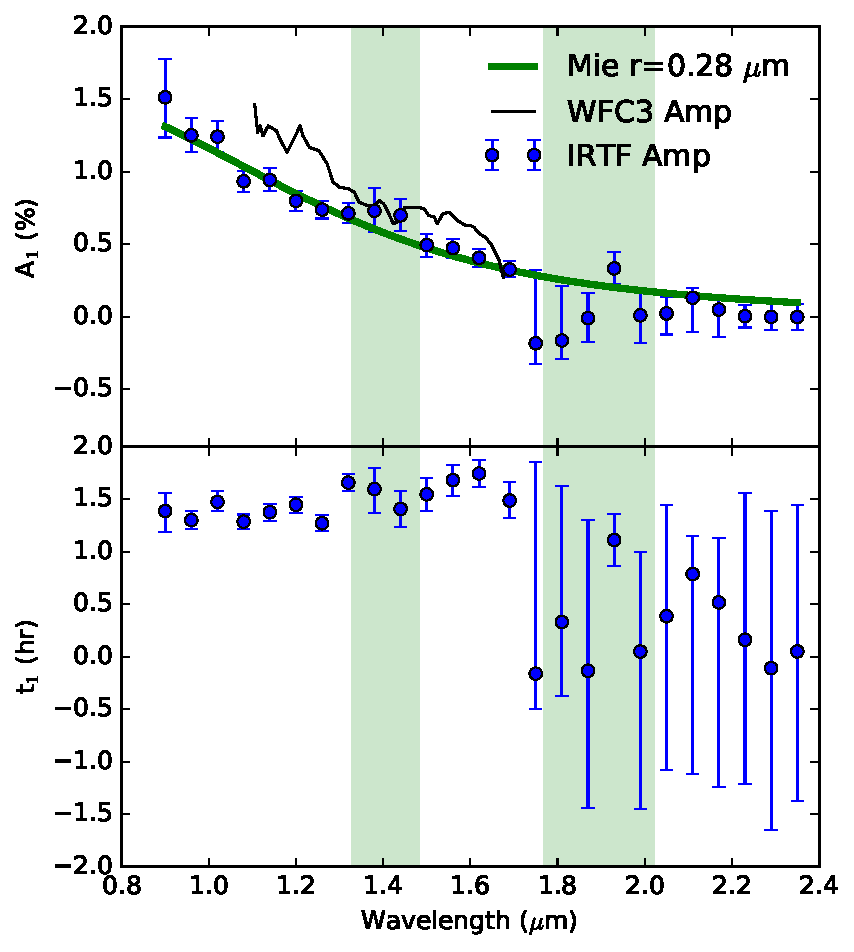
\includegraphics[width=0.5\textwidth]{amp_vs_wavl_j1821.pdf}
	\label{fig:ampspec1821}
	}
	\caption{Sine fit amplitude versus wavelength for each brown dwarf. The regions at 1.4~$\mu$m and 1.9~$\mu$m (shaded with a salmon color) are contaminated by telluric absorption so the variations can likely be due to telluric variability not corrected by the reference star. 2MASS J0835 shows no clear trend in wavelength, while 2MASS J1821 has a strong slope indicative of Mie-scattering particles.}
	\label{fig:ampSpec}
\end{figure*} 

\begin{figure}
\begin{centering}
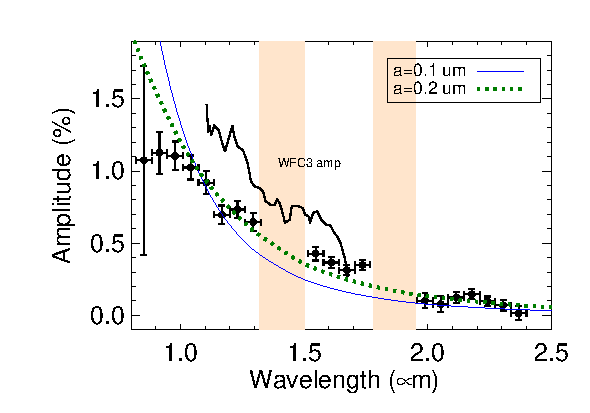
\includegraphics[width=0.5\textwidth]{images/mie_fits/amp_vs_wavl_j1821_mie_sc.pdf}
\caption{Amplitude spectrum using the \texttt{IDL} fits and holding the rotational period fixed at the literature value.
Representative Mie-scattering models are shown for a particle size distribution of 0.1$\mu$m and 0.2$\mu$m pyroxene grains.}\label{fig:IDLmieScatterA1821}
\end{centering}
\end{figure}


%If  used, this work made use of the \texttt{astropy} package \citep{astropy2013}.
%If used, some data was collected from the Open Exoplanet Catalogue \citep{rein2012openExoCat}.

%% In a manner similar to \objectname authors can provide links to dataset
%% hosted at participating data centers via the \dataset{} command.  The
%% second curly bracket argument is printed in the text while the first
%% parentheses argument serves as the valid data set identifier.  Large
%% lists of data set are best provided in a table (see Table 3 for an example).
%% Valid data set identifiers should be obtained from the data center that
%% is currently hosting the data.
%%
%% Note that AASTeX interprets everything between the curly braces in the 
%% macro as regular text, so any special characters, e.g. "#" or "_," must be 
%% preceded by a backslash. Otherwise, you will get a LaTeX error when you 
%% compile your manuscript.  Special characters do not 
%% need to be escaped in the optional, square-bracket argument.



%% In this section, we use  the \subsection command to set off
%% a subsection.  \footnote is used to insert a footnote to the text.

%% Observe the use of the LaTeX \label
%% command after the \subsection to give a symbolic KEY to the
%% subsection for cross-referencing in a \ref command.
%% You can use LaTeX's \ref and \label commands to keep track of
%% cross-references to sections, equations, tables, and figures.
%% That way, if you change the order of any elements, LaTeX will
%% automatically renumber them.

%% This section also includes several of the displayed math environments
%% mentioned in the Author Guide.


%% The equation environment wil produce a numbered display equation.


%% The \notetoeditor{TEXT} command allows the author to communicate
%% information to the copy editor.  This information will appear as a
%% footnote on the printed copy for the manuscript style file.  Nothing will
%% appear on the printed copy if the preprint or
%% preprint2 style files are used.

%% The eqnarray environment produces multi-line display math. The end of
%% each line is marked with a \\. Lines will be numbered unless the \\
%% is preceded by a \nonumber command.
%% Alignment points are marked by ampersands (&). There should be two
%% ampersands (&) per line.

%% Putting eqnarrays or equations inside the mathletters environment groups
%% the enclosed equations by letter. For instance, the eqnarray below, instead
%% of being numbered, say, (4) and (5), would be numbered (4a) and (4b).
%% LaTeX the paper and look at the output to see the results.

%% This section contains more display math examples, including unnumbered
%% equations (displaymath environment). The last paragraph includes some
%% examples of in-line math featuring a couple of the AASTeX symbol macros.

%% The displaymath environment will produce the same sort of equation as
%% the equation environment, except that the equation will not be numbered
%% by LaTeX.
%% If you wish to include an acknowledgments section in your paper,
%% separate it off from the body of the text using the \acknowledgments
%% command.

%% Included in this acknowledgments section are examples of the
%% AASTeX hypertext markup commands. Use \url without the optional [HREF]
%% argument when you want to print the url directly in the text. Otherwise,
%% use either \url or \anchor, with the HREF as the first argument and the
%% text to be printed in the second.

\acknowledgments



%% To help institutions obtain information on the effectiveness of their
%% telescopes, the AAS Journals has created a group of keywords for telescope
%% facilities. A common set of keywords will make these types of searches
%% significantly easier and more accurate. In addition, they will also be
%% useful in linking papers together which utilize the same telescopes
%% within the framework of the National Virtual Observatory.
%% See the AASTeX Web site at http://aastex.aas.org/
%% for information on obtaining the facility keywords.

%% After the acknowledgments section, use the following syntax and the
%% \facility{} macro to list the keywords of facilities used in the research
%% for the paper.  Each keyword will be checked against the master list during
%% copy editing.  Individual instruments or configurations can be provided 
%% in parentheses, after the keyword, but they will not be verified.

%{\it Facilities:} \facility{Nickel}, \facility{HST (STIS)}, \facility{CXO (ASIS)}.

%% Appendix material should be preceded with a single \appendix command.
%% There should be a \section command for each appendix. Mark appendix
%% subsections with the same markup you use in the main body of the paper.

%% Each Appendix (indicated with \section) will be lettered A, B, C, etc.
%% The equation counter will reset when it encounters the \appendix
%% command and will number appendix equations (A1), (A2), etc.

%\appendix


%% The reference list follows the main body and any appendices.
%% Use LaTeX's thebibliography environment to mark up your reference list.
%% Note \begin{thebibliography} is followed by an empty set of
%% curly braces.  If you forget this, LaTeX will generate the error
%% "Perhaps a missing \item?".
%%
%% thebibliography produces citations in the text using \bibitem-\cite
%% cross-referencing. Each reference is preceded by a
%% \bibitem command that defines in curly braces the KEY that corresponds
%% to the KEY in the \cite commands (see the first section above).
%% Make sure that you provide a unique KEY for every \bibitem or else the
%% paper will not LaTeX. The square brackets should contain
%% the citation text that LaTeX will insert in
%% place of the \cite commands.

%% We have used macros to produce journal name abbreviations.
%% AASTeX provides a number of these for the more frequently-cited journals.
%% See the Author Guide for a list of them.

%% Note that the style of the \bibitem labels (in []) is slightly
%% different from previous examples.  The natbib system solves a host
%% of citation expression problems, but it is necessary to clearly
%% delimit the year from the author name used in the citation.
%% See the natbib documentation for more details and options.

\bibliographystyle{apj}
\bibliography{bd_biblio}

%\clearpage

%% Use the figure environment and \plotone or \plottwo to include
%% figures and captions in your electronic submission.
%% To embed the sample graphics in
%% the file, uncomment the \plotone, \plottwo, and
%% \includegraphics commands
%%
%% If you need a layout that cannot be achieved with \plotone or
%% \plottwo, you can invoke the graphicx package directly with the
%% \includegraphics command or use \plotfiddle. For more information,
%% please see the tutorial on "Using Electronic Art with AASTeX" in the
%% documentation section at the AASTeX Web site, http://aastex.aas.org/
%%
%% The examples below also include sample markup for submission of
%% supplemental electronic materials. As always, be sure to check
%% the instructions to authors for the journal you are submitting to
%% for specific submissions guidelines as they vary from
%% journal to journal.

%% This example uses \plotone to include an EPS file scaled to
%% 80% of its natural size with \epsscale. Its caption
%% has been written to indicate that additional figure parts will be
%% available in the electronic journal.

%\begin{figure}
%\epsscale{.80}
%\plotone{f1.eps}
%\caption{Derived spectra for 3C138 \citep[see][]{heiles03}. Plots for all sources are available
%in the electronic edition of {\it The Astrophysical Journal}.\label{fig1}}
%\end{figure}

%\clearpage

%% Here we use \plottwo to present two versions of the same figure,
%% one in black and white for print the other in RGB color
%% for online presentation. Note that the caption indicates
%% that a color version of the figure will be available online.
%%

%\begin{figure}
%\plottwo{f2.eps}{f2_color.eps}
%\caption{A panel taken from Figure 2 of \citet{rudnick03}. 
%See the electronic edition of the Journal for a color version 
%of this figure.\label{fig2}}
%\end{figure}

%% This figure uses \includegraphics to scale and rotate the still frame
%% for an mpeg animation.

%\begin{figure}
%\includegraphics[angle=90,scale=.50]{f3.eps}
%\caption{Animation still frame taken from \citet{kim03}.
%This figure is also available as an mpeg
%animation in the electronic edition of the
%{\it Astrophysical Journal}.}
%\end{figure}

%% If you are not including electonic art with your submission, you may
%% mark up your captions using the \figcaption command. See the
%% User Guide for details.
%%
%% No more than seven \figcaption commands are allowed per page,
%% so if you have more than seven captions, insert a \clearpage
%% after every seventh one.

%% Tables should be submitted one per page, so put a \clearpage before
%% each one.

%% Two options are available to the author for producing tables:  the
%% deluxetable environment provided by the AASTeX package or the LaTeX
%% table environment.  Use of deluxetable is preferred.
%%

%% Three table samples follow, two marked up in the deluxetable environment,
%% one marked up as a LaTeX table.

%% In this first example, note that the \tabletypesize{}
%% command has been used to reduce the font size of the table.
%% We also use the \rotate command to rotate the table to
%% landscape orientation since it is very wide even at the
%% reduced font size.
%%
%% Note also that the \label command needs to be placed
%% inside the \tablecaption.

%% This table also includes a table comment indicating that the full
%% version will be available in machine-readable format in the electronic
%% edition.

%% If you use the table environment, please indicate horizontal rules using
%% \tableline, not \hline.
%% Do not put multiple tabular environments within a single table.
%% The optional \label should appear inside the \caption command.



%% If the table is more than one page long, the width of the table can vary
%% from page to page when the default \tablewidth is used, as below.  The
%% individual table widths for each page will be written to the log file; a
%% maximum tablewidth for the table can be computed from these values.
%% The \tablewidth argument can then be reset and the file reprocessed, so
%% that the table is of uniform width throughout. Try getting the widths
%% from the log file and changing the \tablewidth parameter to see how
%% adjusting this value affects table formatting.

%% The \dataset{} macro has also been applied to a few of the objects to
%% show how many observations can be tagged in a table.


%% Tables may also be prepared as separate files. See the accompanying
%% sample file table.tex for an example of an external table file.
%% To include an external file in your main document, use the \input
%% command. Uncomment the line below to include table.tex in this
%% sample file. (Note that you will need to comment out the \documentclass,
%% \begin{document}, and \end{document} commands from table.tex if you want
%% to include it in this document.)

%% \input{table}

%% The following command ends your manuscript. LaTeX will ignore any text
%% that appears after it.

\end{document}

%%
%% End of file `sample.tex'.
